% --------------- PLANTILLA MAXI (GOD) -----------------
\documentclass[11pt, twocolumn]{article}

\usepackage[latin1,utf8]{inputenc}
\usepackage{verbatim}
\usepackage{multirow}
\usepackage{float}
\usepackage{enumerate}
\usepackage{graphics,graphicx,xcolor}
\usepackage{subfig}
\usepackage[spanish,es-tabla]{babel}
\usepackage{caption}
\usepackage{placeins}
\usepackage{afterpage}
\usepackage{blindtext}
\usepackage{multicol}
\usepackage{geometry}
\usepackage{lipsum}

%paquete para referencias
\usepackage[backend=biber, style=nature, citestyle=numeric, sorting=none, maxbibnames=99]{biblatex} % 
% \usepackage{natbib}
% \bibliographystyle{apsrev4-1} % Utiliza el archivo .bst de APS o uno similar

\usepackage{titling} % Paquete para personalizar título del documento
\usepackage{authblk}  % Paquete para personalizar autores del documento
\renewcommand\Authand{ y } % Reemplazar 'and' con 'y'

\DeclareCaptionFormat{custom}
{%
    \textbf{#1#2}\textit{\small #3}
}
\captionsetup{format=custom}

\newgeometry{bottom=3cm, top=2cm, left=3cm, right=3cm}
\usepackage{hyperref}
\hypersetup{
  colorlinks   = true, %Colours links instead of ugly boxes
  urlcolor     = blue, %Colour for external hyperlinks
  linkcolor    = black, %Colour of internal links
  citecolor   = black %Colour of citations
}

%paquete para unidades
\usepackage{siunitx}
% seteo punto como separador decimal
\AtBeginDocument{\decimalpoint}


% \DeclareSIUnit\torr{Torr}

%% Paquetes de la AMS
\usepackage{amsmath, amsthm, amsfonts, amssymb}

%componentes de texto
\usepackage{textcomp}


% Personaliza título del documento
\pretitle{\begin{center}\LARGE\bfseries}
    \posttitle{\par\vspace{0.5em}\end{center}\large}
    \preauthor{\begin{center}\large \lineskip 0.8em \begin{tabular}[t]{c}}
    \postauthor{\end{tabular}\par\end{center}}
    \predate{\begin{center}\large}
    \postdate{\par\end{center}}


\usepackage{fancyhdr}
\pagestyle{fancy}

% Definimos el encabezado de las paginas pares e impares.
\lhead{IMÁGENES MÉDICAS}
\chead{Práctica 4 - 2024}
\rhead{Gatto Maximiliano}
\renewcommand{\headrulewidth}{0.5pt}

% aqui definimos el pie de pagina de las paginas pares e impares.
\lfoot[a1]{}
\cfoot[c1]{\thepage}
\rfoot[e1]{}

\renewcommand{\footrulewidth}{0.5pt}

% ------------------- TITULO ----------------------
% \title{\textbf{Procesamiento de imágenes digitales} \\ \vspace{1cm} \large IMÁGENES MÉDICAS - Práctica 2 - 2024}

\title{{\large IMÁGENES MÉDICAS - Práctica 4 - 2024} \\ \vspace{1cm}\textbf{Reconstrucción de Imágenes Tomográficas: Métodos Iterativos}}



\author[ ]{\textbf{Maximiliano Gatto}}
\affil[ ]{Instituto Balseiro (UNCuyo - CNEA) - Bariloche, Río Negro, Argentina\vspace{0.4cm}}
\affil[ ]{\href{mailto:maximiliano.gatto@ib.edu.ar}{maximiliano.gatto@ib.edu.ar}}

\date{\today}

\begin{document}
\maketitle

% ------------------ INTRODUCCION ---------------------
\section{Introducción}
En esta práctica, se exploraron métodos algebraicos para reconstruir imágenes tomográficas a partir de proyecciones o sinogramas, incluyendo algoritmos como \textit{Kaczmarz} o \textit{ART (Algebraic Reconstruction Technique)}, y variantes como \textit{Kaczmarz simétrico}, \textit{Kaczmarz aleatorio} y \textit{SART (Simultaneous ART)}. También se implementó el algoritmo de \textit{Expectation Maximization}, común en la reconstrucción de imágenes PET. Se evaluaron diferentes métricas de precisión utilizando scripts en \texttt{Python} y \texttt{Matlab}, disponibles en el siguiente enlace.

% ------------------ RESULTADOS ---------------------
\section{Resultados}

% --------------- EJ 1 ---------------------
\subsection*{Ejercicio 1}
En este ejercicio, se llevó a cabo la técnica de reconstrucción algebraica (ART). Esta técnica implica medir y estimar proyecciones, luego dividir el resultado por el número de píxeles en una dirección específica. La iteración que rige el algoritmo se describe mediante la siguiente ecuación:

\begin{equation}  \label{eq:ART}
  f^{(k+1)}_j = f^{(k)}_j + \frac{p_i - \sum_{j=1}^N f_{ji}^{(k)}}{N}
\end{equation}

\noindent donde $p_i$ es el número de cuentas en la dirección $i$, $N$ es el número de detectores en cada dirección, $f^{(k)}_j$ es el valor actual del píxel $j$, $f^{(k+1)}_j$ es el valor actualizado, y $\sum_{j=1}^N f_{ji}^{(k)}$ es la suma de los $N$ píxeles en la dirección $i$.

Se aplicó el método ART a una imagen de tamaño $2\times2$, que se muestra en la Figura \ref{fig:ej_1_orig}, iterando sobre todas las direcciones.

\begin{figure}[htbp]
  \centering
  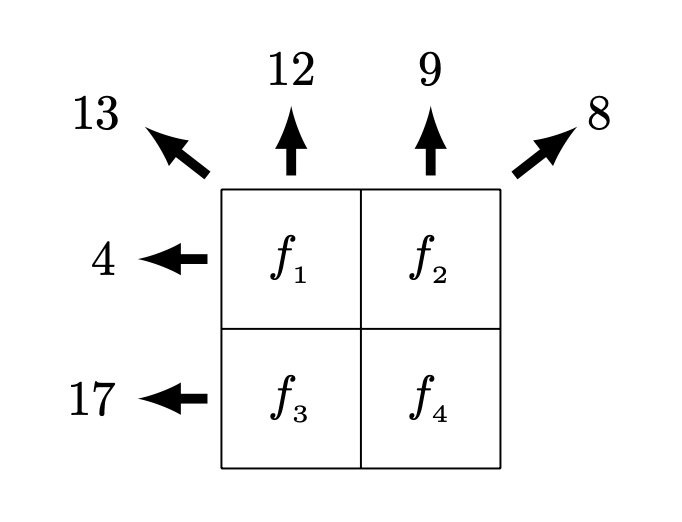
\includegraphics[width=0.45\textwidth]{images/ej_1/original_p1.png}
  \caption{imagen de tamaño $2\times2$ para reconstruir utilizando el algoritmo ART.}
  \label{fig:ej_1_orig}
\end{figure}

Denominando $\vec{p}  = (17, 4, 13, 12, 9, 8)$ a las proyecciones medidas, se inició el algoritmo (Ecuación \ref{eq:ART}) con una imagen inicial de ceros e iterando sobre las direcciones verticales, horizontales y finalmente las oblicuas. Los resultados obtenidos para cada caso de detallan a continuación.

\textbf{Dirección vertical:}

\begin{eqnarray*}
  f_1^{(1)} = f_1^{(0)} + \frac{p_4 - (f_1^{(0)}+f_3^{(0)})}{N} =  6 \\
  f_2^{(1)} = f_2^{(0)} + \frac{p_5 - (f_2^{(0)}+f_4^{(0)})}{N} = \frac{9}{2}\\
  f_3^{(1)} = f_3^{(0)} + \frac{p_4 - (f_1^{(0)}+f_3^{(0)})}{N} = 6 \\
  f_4^{(1)} = f_4^{(0)} + \frac{p_5 - (f_2^{(0)}+f_4^{(0)})}{N} = \frac{9}{2}
\end{eqnarray*}


\textbf{Dirección horizontal:}
\begin{eqnarray*}
  f_1^{(2)} = f_1^{(1)} + \frac{p_2 - (f_1^{(1)}+f_2^{(1)})}{N} = \frac{11}{4} \\
  f_2^{(2)} = f_2^{(1)} + \frac{p_2 - (f_1^{(1)}+f_2^{(1)})}{N} = \frac{5}{4}\\
  f_3^{(2)} = f_3^{(1)} + \frac{p_1 - (f_3^{(1)}+f_4^{(1)})}{N} = \frac{37}{4} \\
  f_4^{(2)} = f_4^{(1)} + \frac{p_1 - (f_3^{(1)}+f_4^{(1)})}{N} = \frac{31}{4}
\end{eqnarray*}

\textbf{Dirección oblicua:}
\begin{eqnarray*}
  f_1^{(3)} = f_1^{(2)} + \frac{p_3 - (f_1^{(2)}+f_4^{(2)})}{N} = 4 \\
  f_2^{(3)} = f_2^{(2)} + \frac{p_6 - (f_2^{(2)}+f_3^{(2)})}{N} = 0\\
  f_3^{(3)} = f_3^{(2)} + \frac{p_6 - (f_2^{(2)}+f_3^{(2)})}{N} = 8 \\
  f_4^{(2)} = f_4^{(2)} + \frac{p_3 - (f_1^{(2)}+f_4^{(2)})}{N} = 9
\end{eqnarray*}

Notar que, luego de estas iteraciones, la imagen reconstruida se corresponde con el número de cuentas en cada dirección, por lo que se puede concluir que el algoritmo convergió a la imagen original. La imagen resultante se muestra en la Figura \ref{fig:ej_1_rec}.

\begin{figure}[htbp]
  \centering
  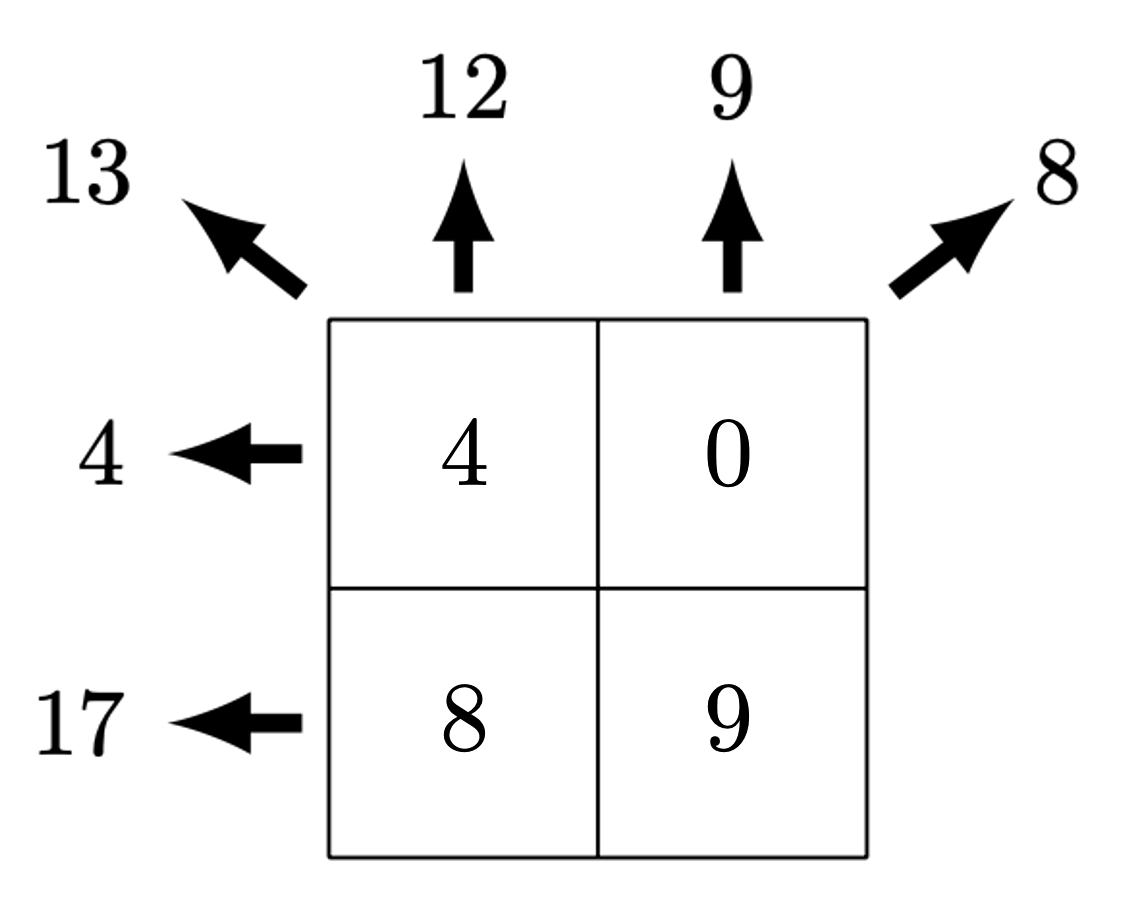
\includegraphics[width=0.4\textwidth]{images/ej_1/imagen_resconstruida_ej1.png}
  \caption{imagen reconstruida utilizando el algoritmo ART.}
  \label{fig:ej_1_rec}
\end{figure}

\subsection*{Ejercicio 2}
Se implementó el algoritmo \textit{ART} para la reconstrucción de la imagen. Se importó una imagen desde un archivo de \texttt{Matlab} \texttt{XCAT512.mat}, pero se ejecutó el código en \texttt{Python} utilizando la función \texttt{loadmat} del paquete \href{https://docs.scipy.org/doc/scipy/reference/io.html}{\texttt{scipy.io}}. La imagen original se muestra en la Figura \ref{fig:ej_2_orig}.

\begin{figure} [htbp]
  \centering
  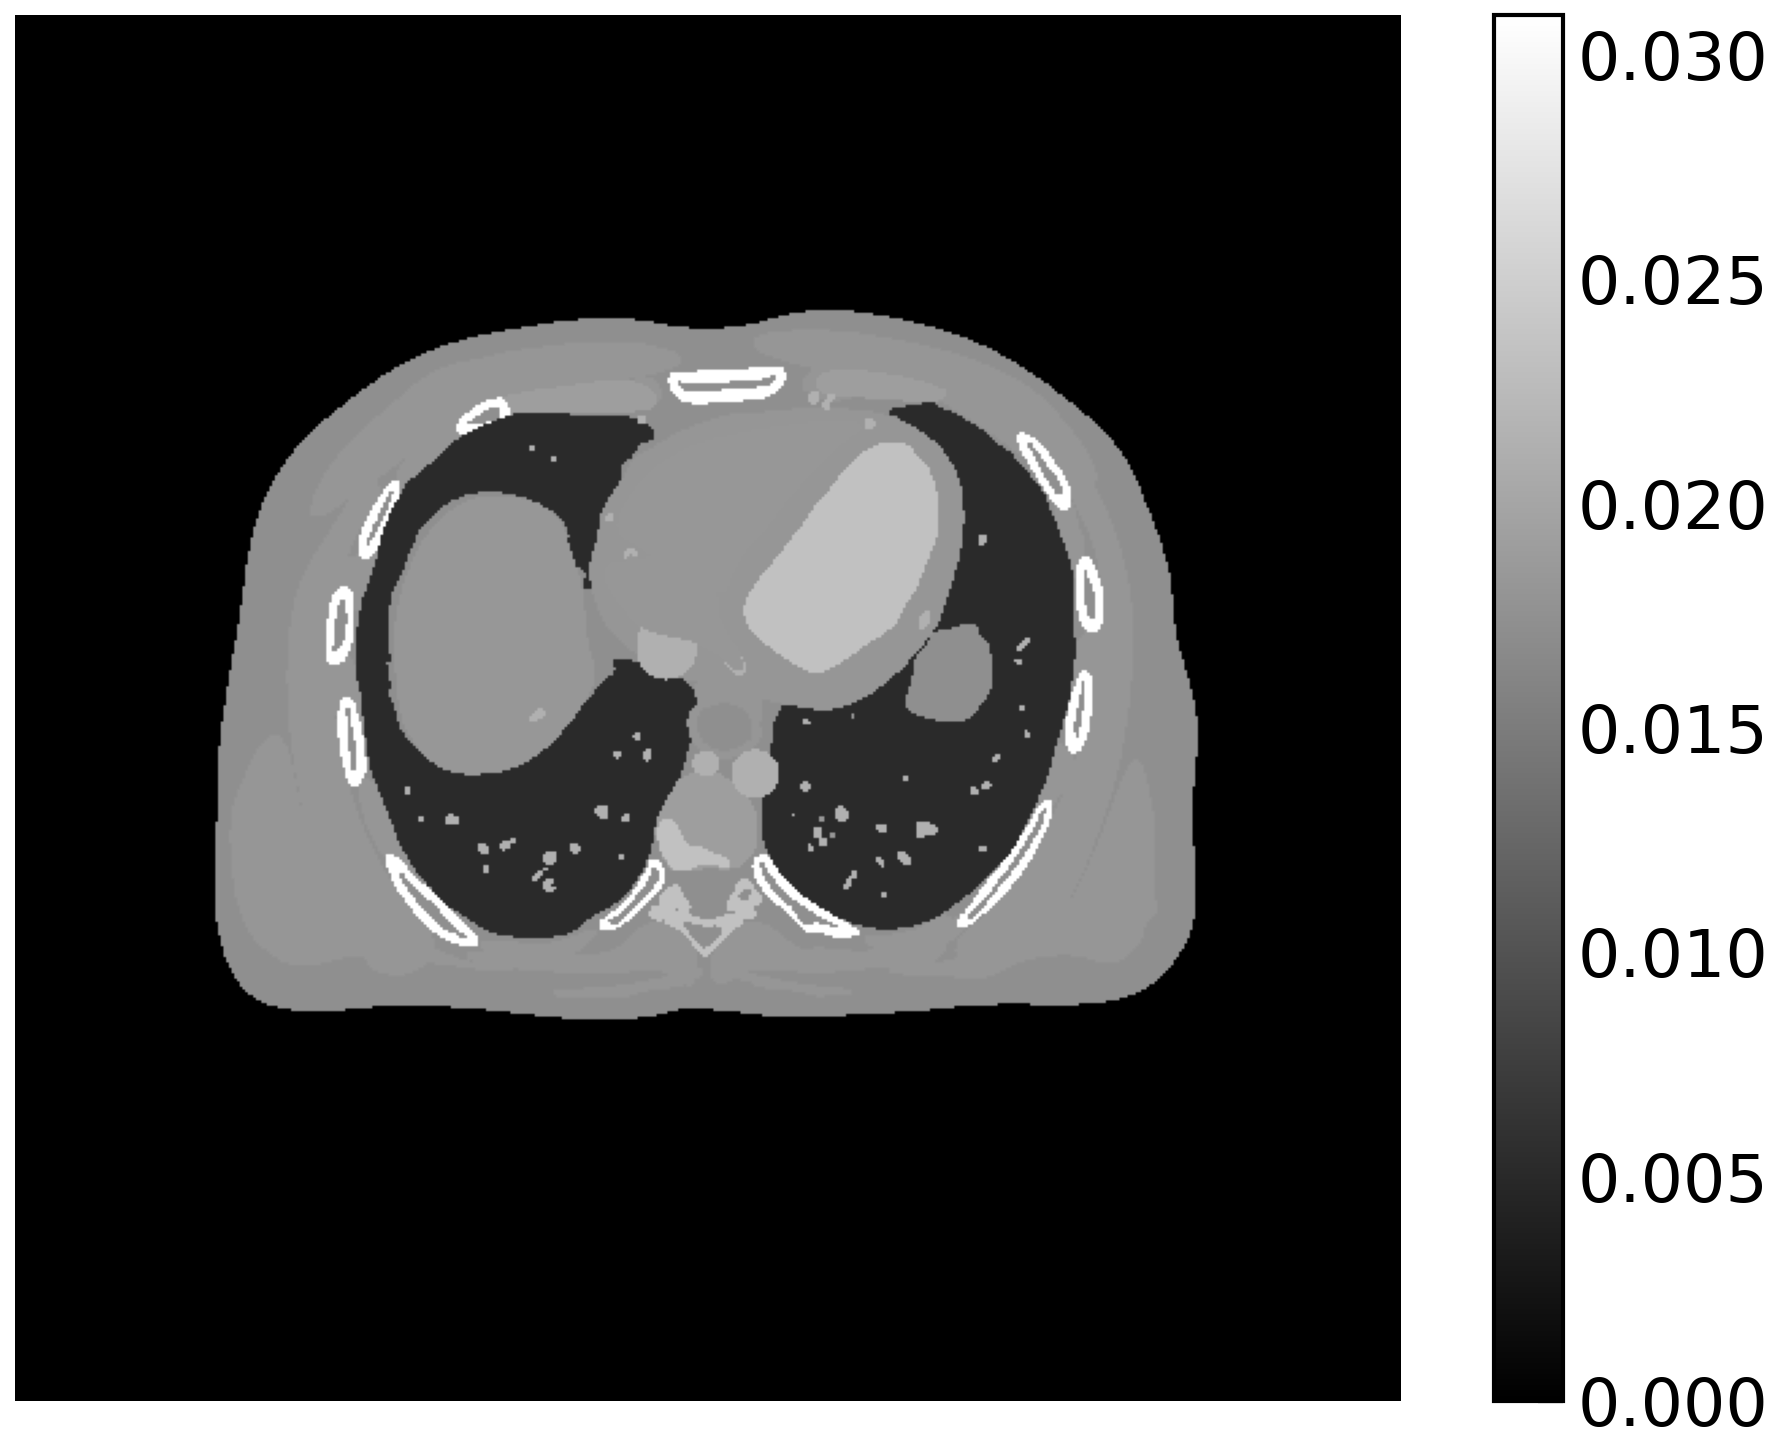
\includegraphics[width=0.45\textwidth]{images/ej_2/original_ej_2.png}
  \caption{imagen original de tamaño $512\times512$ utilizada para la reconstrucción.}
  \label{fig:ej_2_orig}
\end{figure}

Se validó el algoritmo de reconstrucción generando un sinograma con la transformada de Radon (implementada en \href{https://scikit-image.org/docs/stable/api/skimage.transform.html#skimage.transform.radon}{\texttt{skimage.transform}}). Se utilizaron $360$ proyecciones y $512$ detectores en cada dirección. La Figura \ref{fig:ej_2_it_200} muestra la reconstrucción después de $200$ iteraciones.

\begin{figure}[htbp]
  \centering
  \subfloat[]{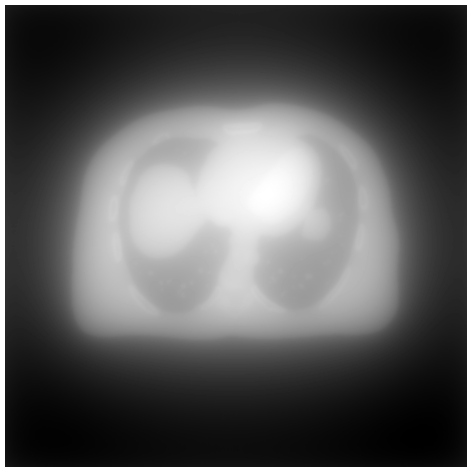
\includegraphics[width=0.24\textwidth]{images/ej_2/200_iter/reconstruccion_artiter_0.png}\label{fig:it_0}}
  \hfill
  \subfloat[]{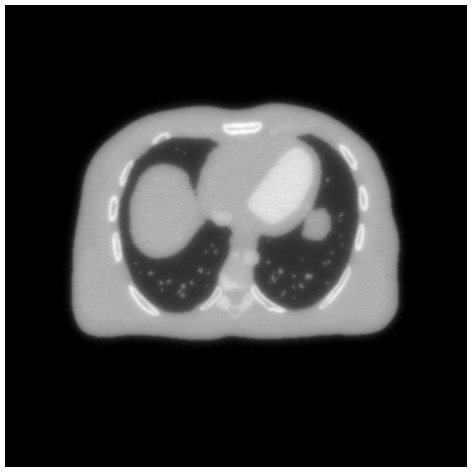
\includegraphics[width=0.24\textwidth]{images/ej_2/200_iter/reconstruccion_artiter_66.png}\label{fig:it_66}}
  \hfill
  \subfloat[]{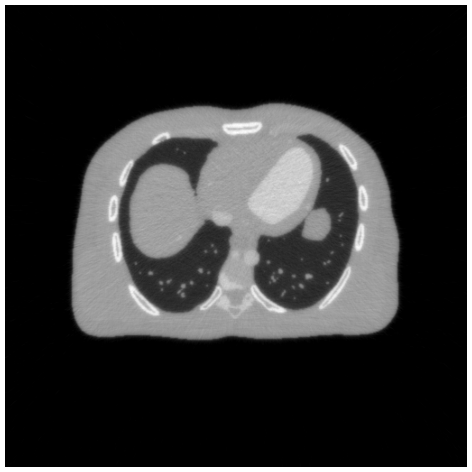
\includegraphics[width=0.24\textwidth]{images/ej_2/200_iter/reconstruccion_artiter_132.png}\label{fig:it_132}}
  \hfill
  \subfloat[]{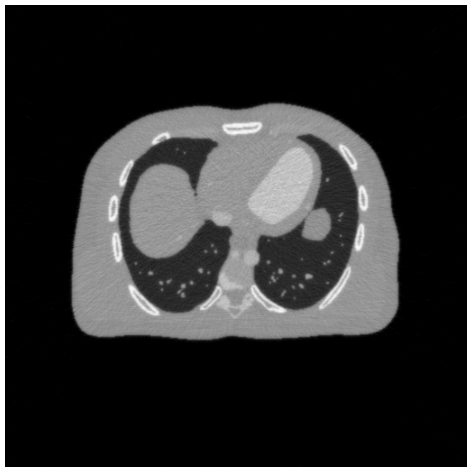
\includegraphics[width=0.24\textwidth]{images/ej_2/200_iter/reconstruccion_artiter_199.png}\label{fig:it_199}}
  \hfill
  \caption{proceso de reconstrucción de la imagen original utilizando el algoritmo ART después de $200$ iteraciones. (a) $1$ iteración, (b) $67$ iteraciones, (c) $133$ iteraciones, (d) $200$ iteraciones.}
  \label{fig:ej_2_it_200}
\end{figure}

Se observa que, luego de $200$ iteraciones, la imagen reconstruida se asemeja a la original (Figura \ref{fig:ej_2_orig}), salvo por algunos artefactos. Además, se aprecia cómo, a medida que aumenta el número de iteraciones, la calidad de la imagen mejora (figuras \ref{fig:it_0}, \ref{fig:it_66}, \ref{fig:it_132} y \ref{fig:it_199}).

Se cuantificaron los errores de reconstrucción del algoritmo \textit{ART} y se los comparó con los obtenidos usando transformada de Radón. Se obtuvo el error cuadrático medio (MSE), la relación entre el pico de la señal y el ruido (PSNR) y el índice de similitud estructural (SSIM). Los resultados se muestran en la Tabla \ref{tab:ej_2_recont}.

\begin{table}[htbp]
  \centering
  \begin{tabular}{|c|c|c|c|}
    \hline
    \textbf{Método} & \textbf{MSE} & \textbf{PSNR} & \textbf{SSIM} \\ \hline
    ART & $1.119\times10^{-2}$ & 29.2432 & 0.99997 \\ \hline
    Radon & $1.526\times10^{-2}$ & 28.1656 & 0.99995 \\ \hline
  \end{tabular}
  \caption{Errores de reconstrucción de la imagen original utilizando el algoritmo ART y la transformada de Radón.}
  \label{tab:ej_2_recont}
\end{table}

Se evaluó la influencia del número de ángulos, detectores y nivel de ruido en el error de reconstrucción del fantoma de \textit{Shepp-Logan} utilizando los métodos \textit{Kaczmarz}, \textit{Kaczmarz simétrico}, \textit{Kaczmarz aleatorio} y \textit{SART}.

Las imágenes se generaron con un script en \texttt{Matlab} con 10 iteraciones, aplicando ruido normal al sinograma (media 0 y varianza 1), multiplicado por una constante ($level$). Se calcularon el MSE, PSNR y SSIM para cada imagen reconstruida. Inicialmente, se fijó el nivel de ruido ($level = 0.01$) y el número de ángulos ($N_\theta = 100$), variando el número de detectores ($N_d$) de 60 a 300. Los resultados se presentan en la Figura \ref{fig:ej_2_detec}.

\begin{figure}[htbp]
  \centering
  \subfloat[]{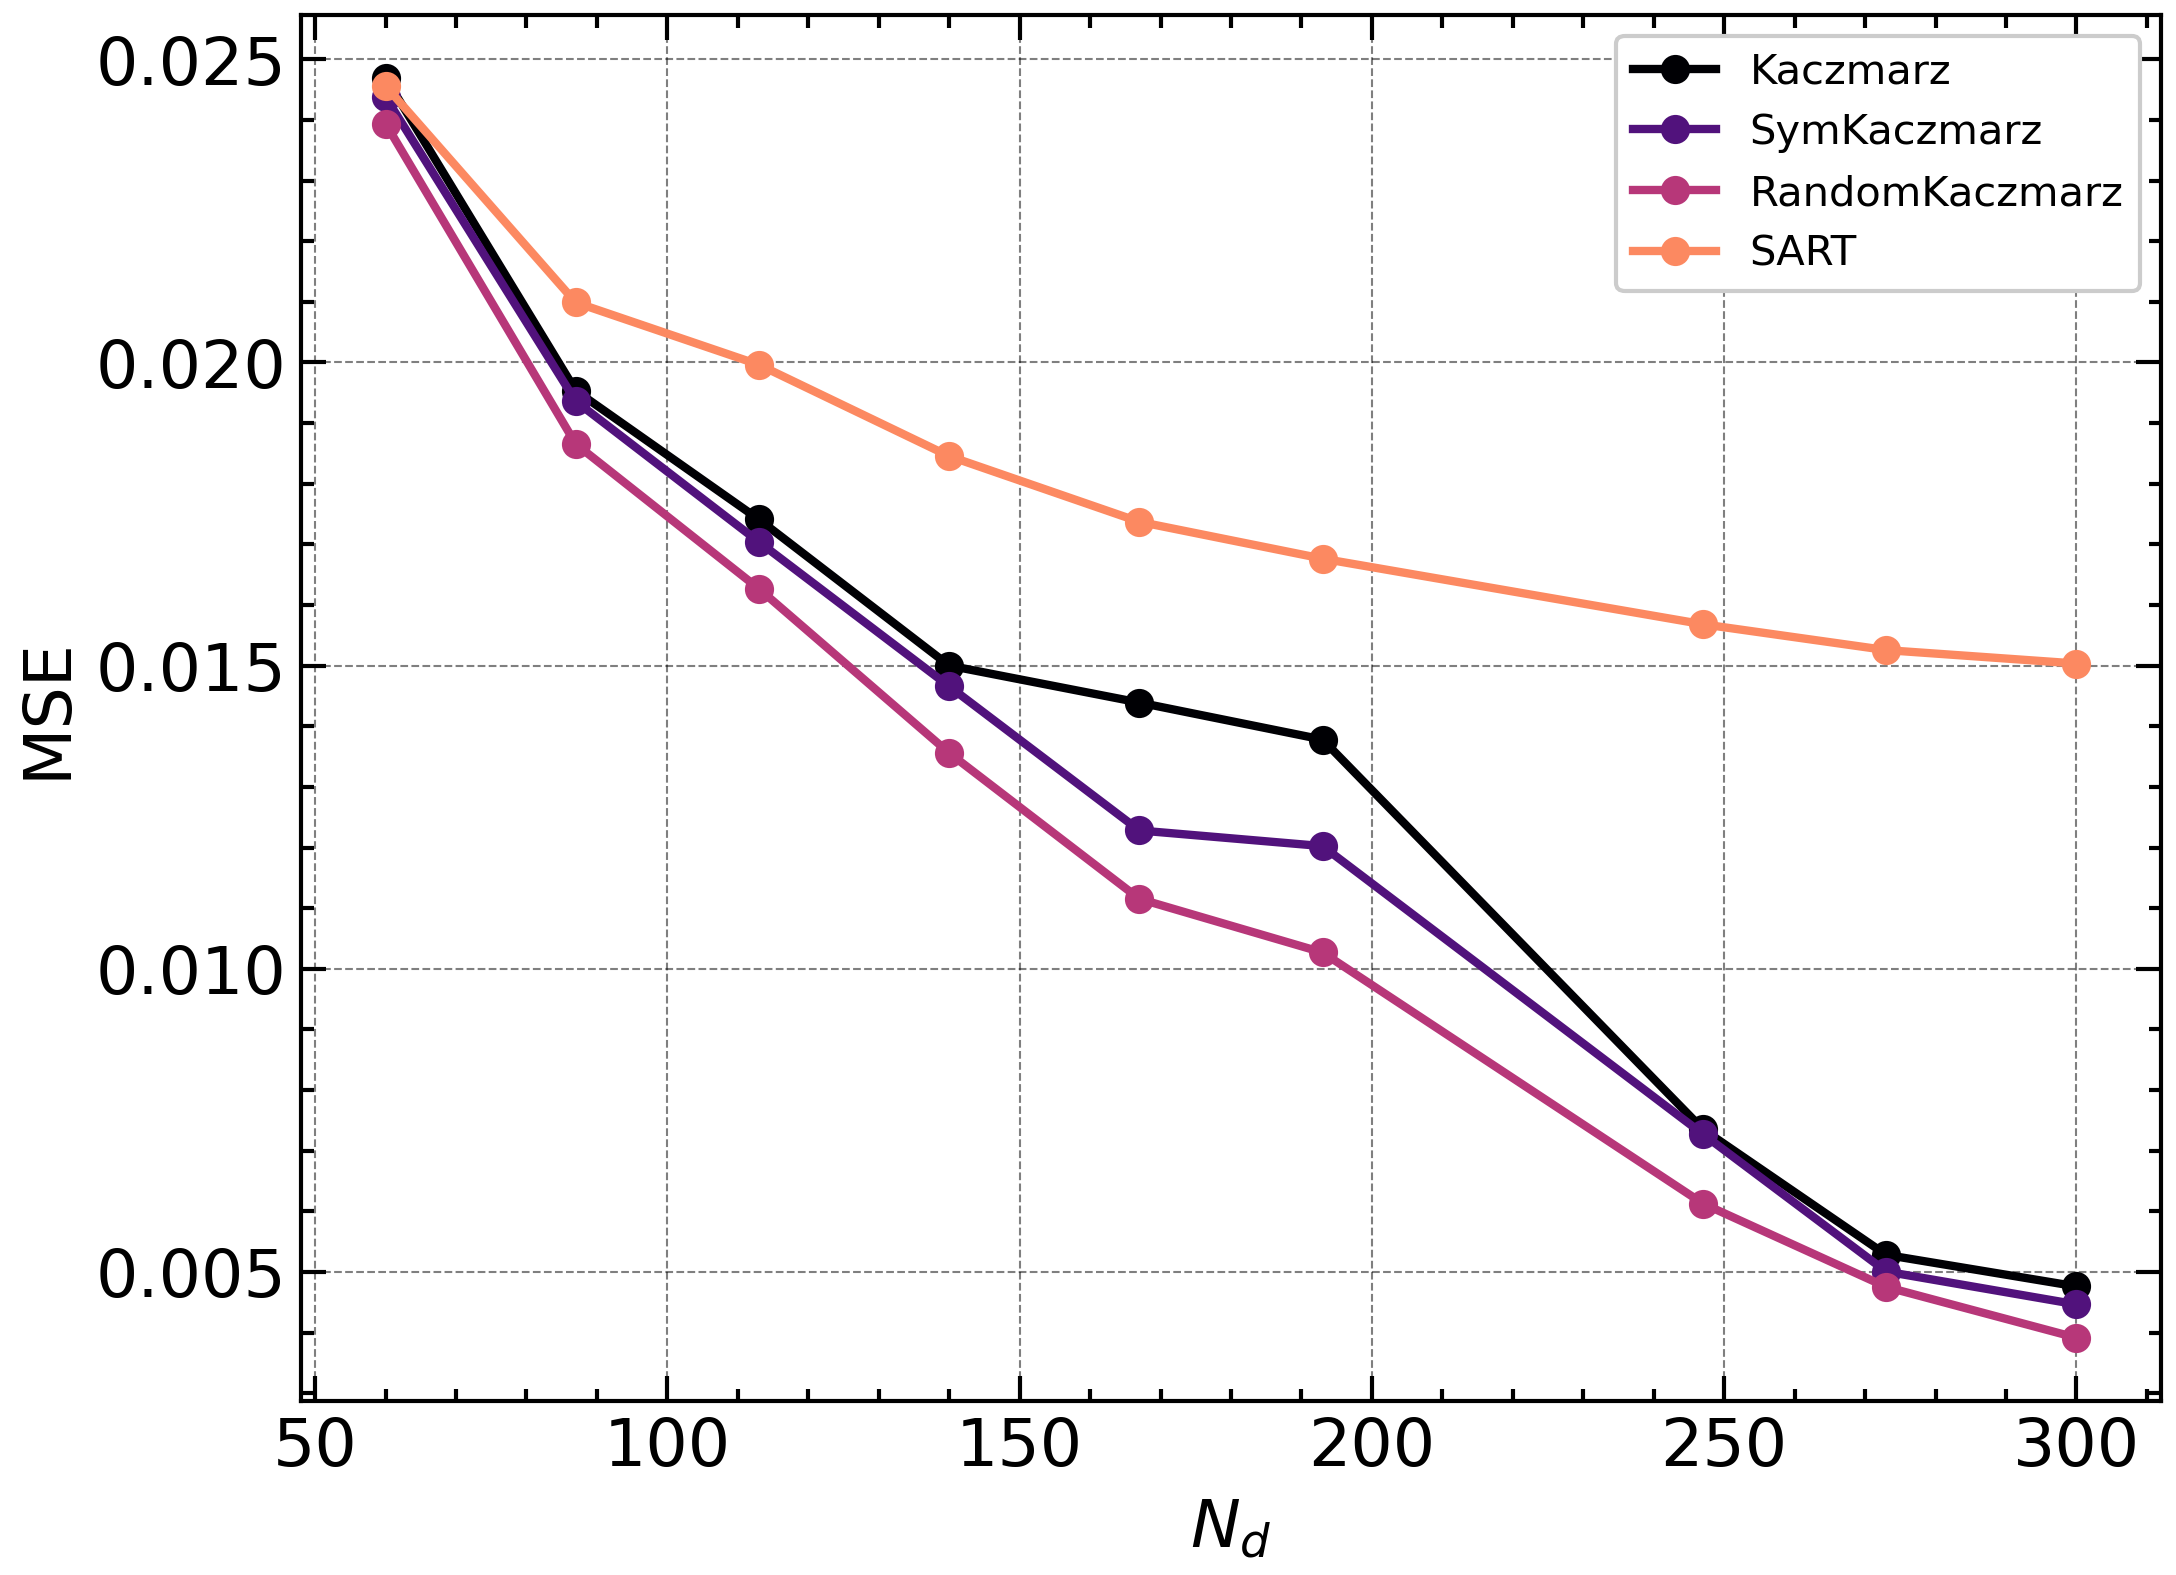
\includegraphics[width=0.45\textwidth]{images/ej_2/detectores/mse.png}\label{fig:mse_detec}}
  \hfill
  \subfloat[]{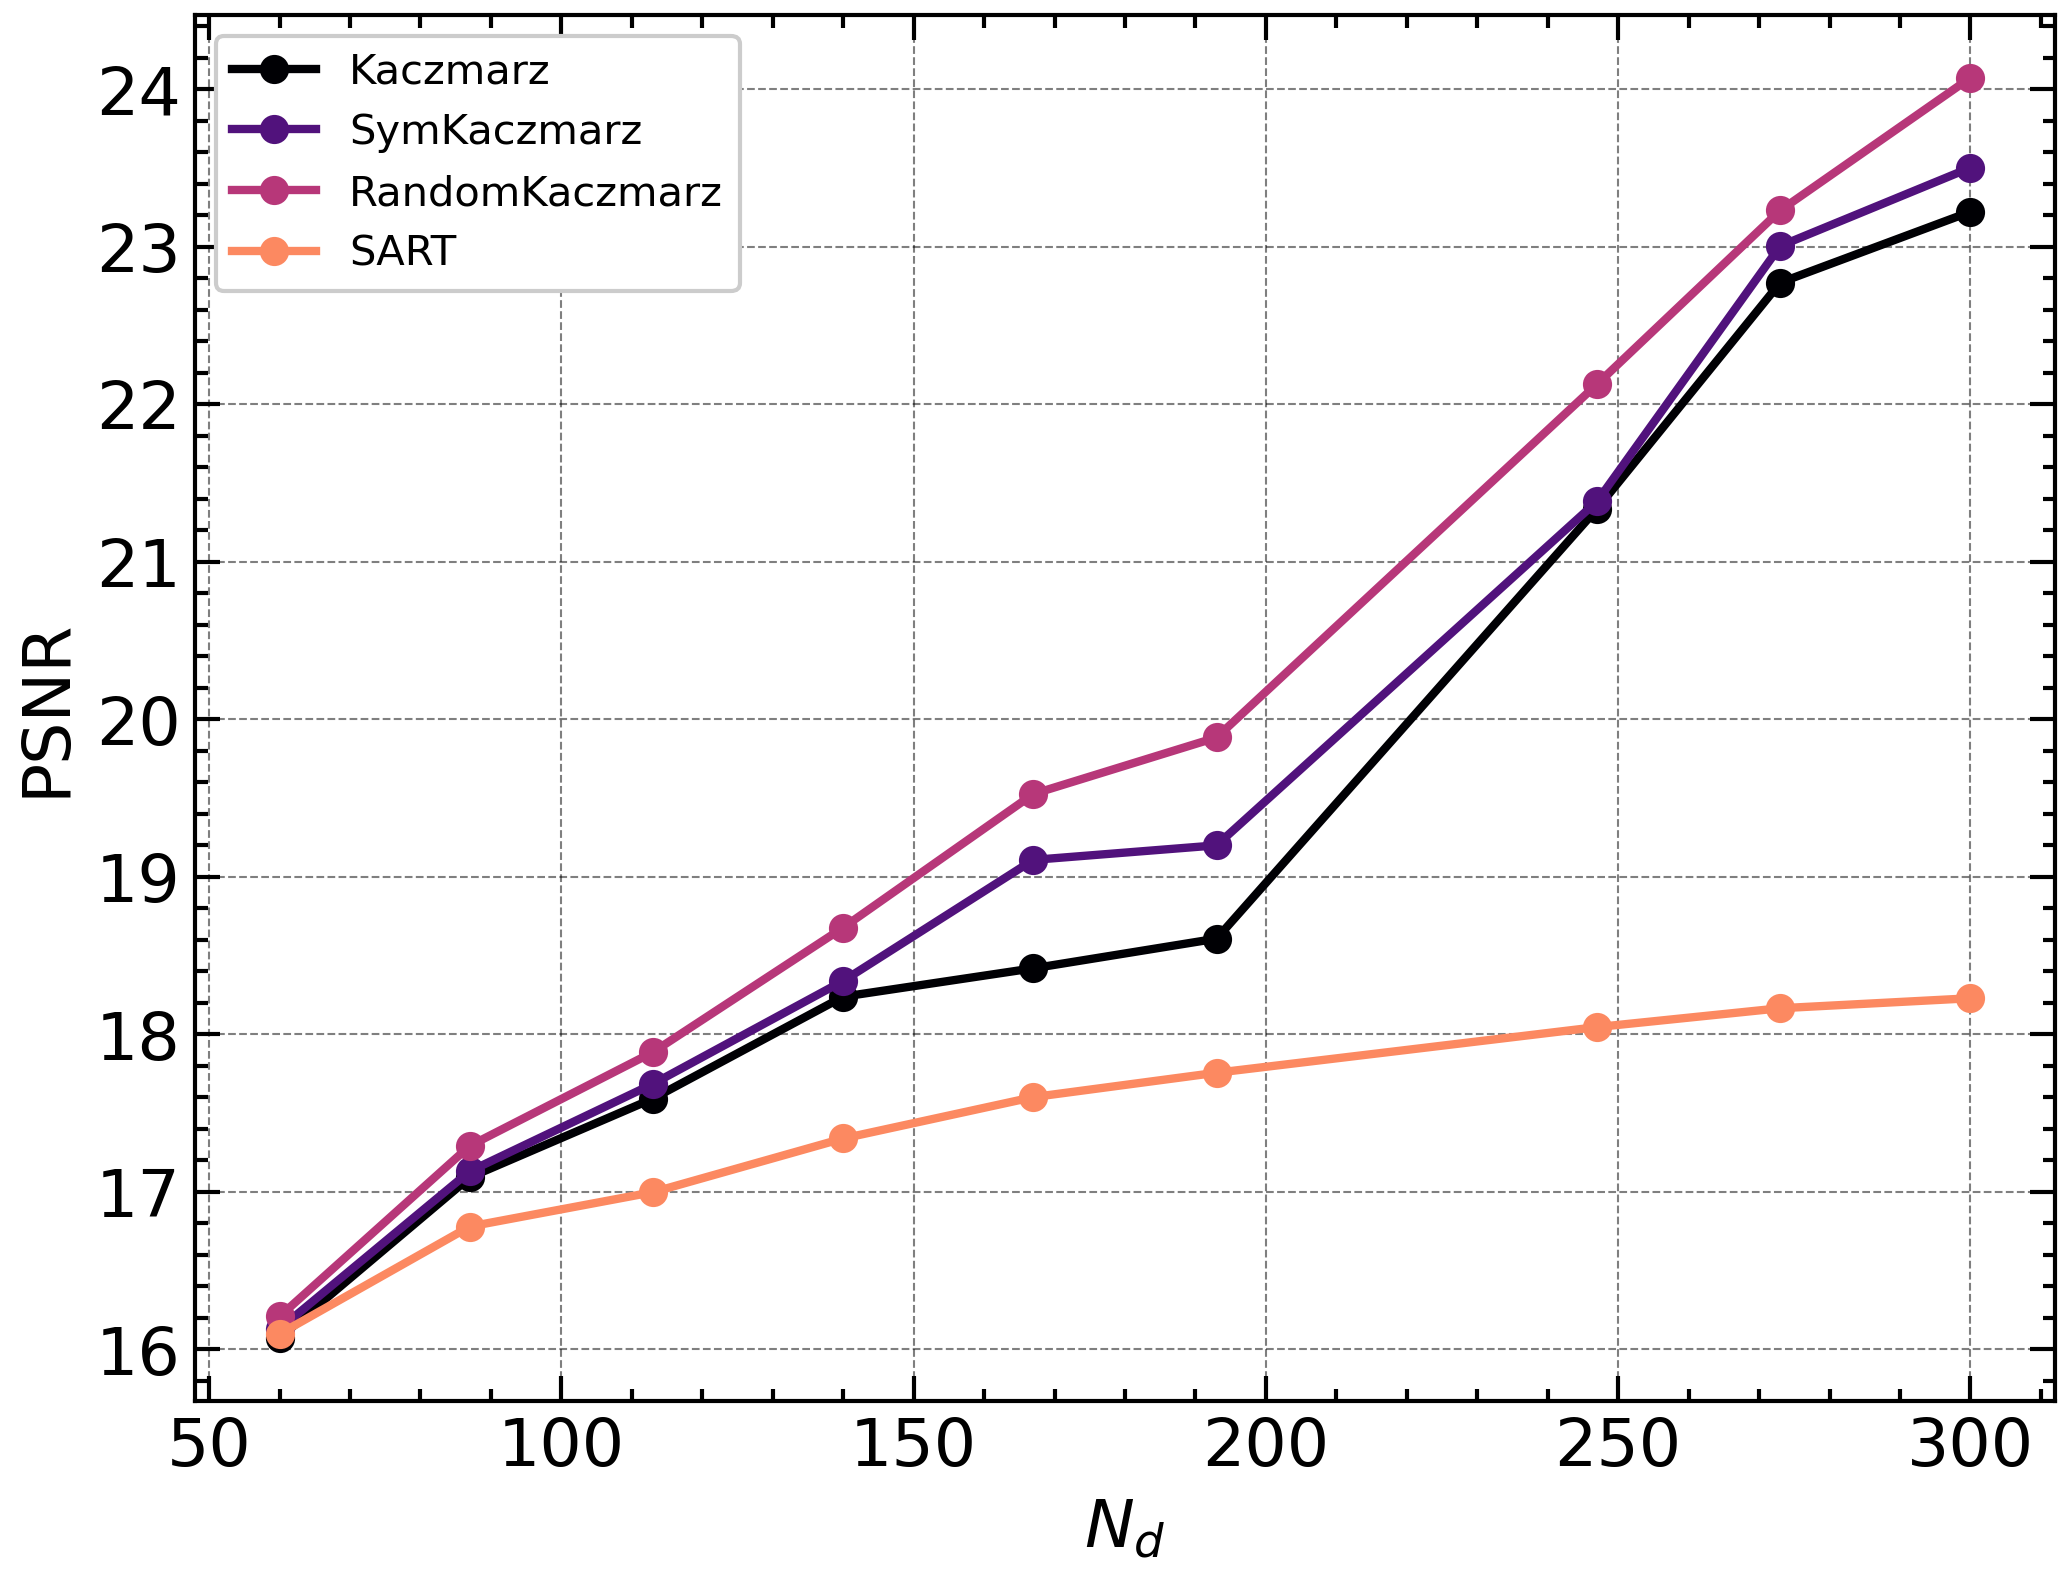
\includegraphics[width=0.42\textwidth]{images/ej_2/detectores/psnr.png}\label{fig:psnr_detec}}
  \hfill
  \subfloat[]{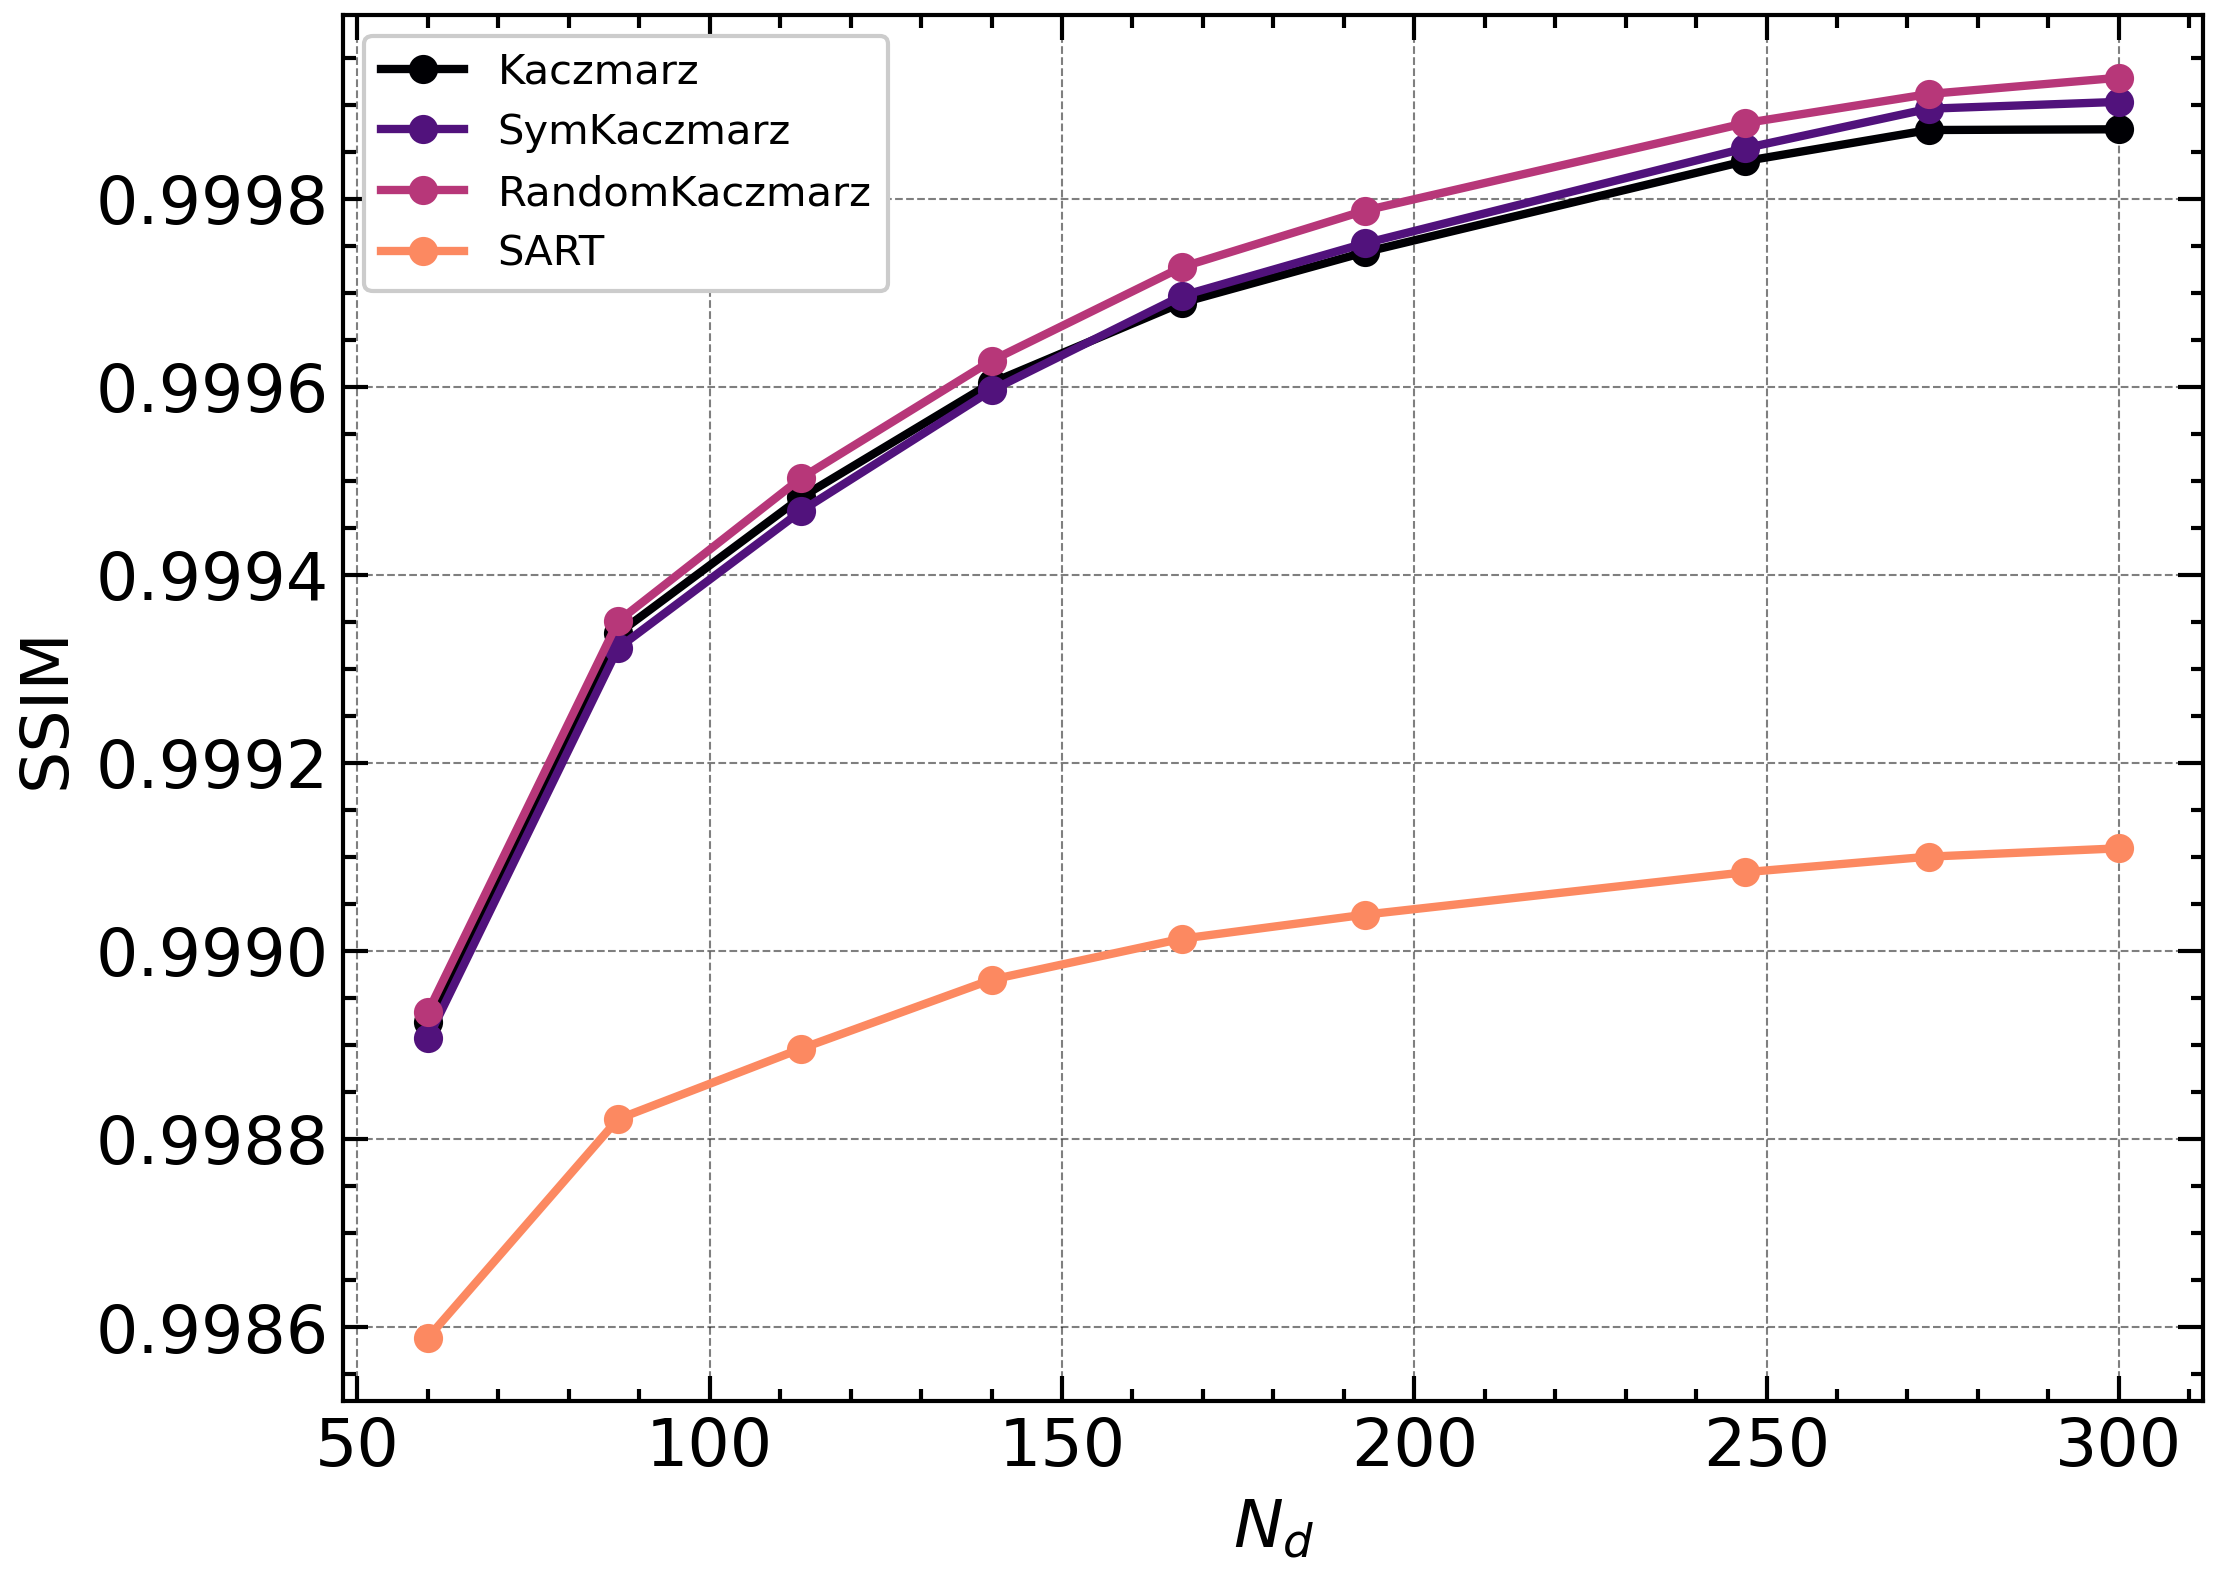
\includegraphics[width=0.45\textwidth]{images/ej_2/detectores/ssim.png}\label{fig:ssim_detec}}
  \hfill
  \caption{error de reconstrucción de la imagen original según el número de detectores ($N_d$). (a) Error cuadrático medio (MSE), (b) relación señal a ruido máxima (PSNR), (c) índice de similitud estructural (SSIM).}
  \label{fig:ej_2_detec}
\end{figure}
En la Figura \ref{fig:ej_2_detec}, se qaprecia que al aumentar los detectores, el error \textit{MSE} disminuye y tanto el \textit{PSNR} como el \textit{SSIM} aumentan, lo que indica una mejor calidad de imagen reconstruida. El algoritmo \textit{SART} sigue esta tendencia pero de manera menos pronunciada, sugiriendo menor sensibilidad al número de detectores. 

En el segundo caso, con nivel de ruido ($level = 0.01$) y detectores fijos ($N_d = 128$), variando el número de ángulos ($N_\theta$) entre 20 y 200, se obtienen resultados que se muestran en la Figura \ref{fig:ej_2_angles}.

\begin{figure}[htbp]
  \centering
  \subfloat[]{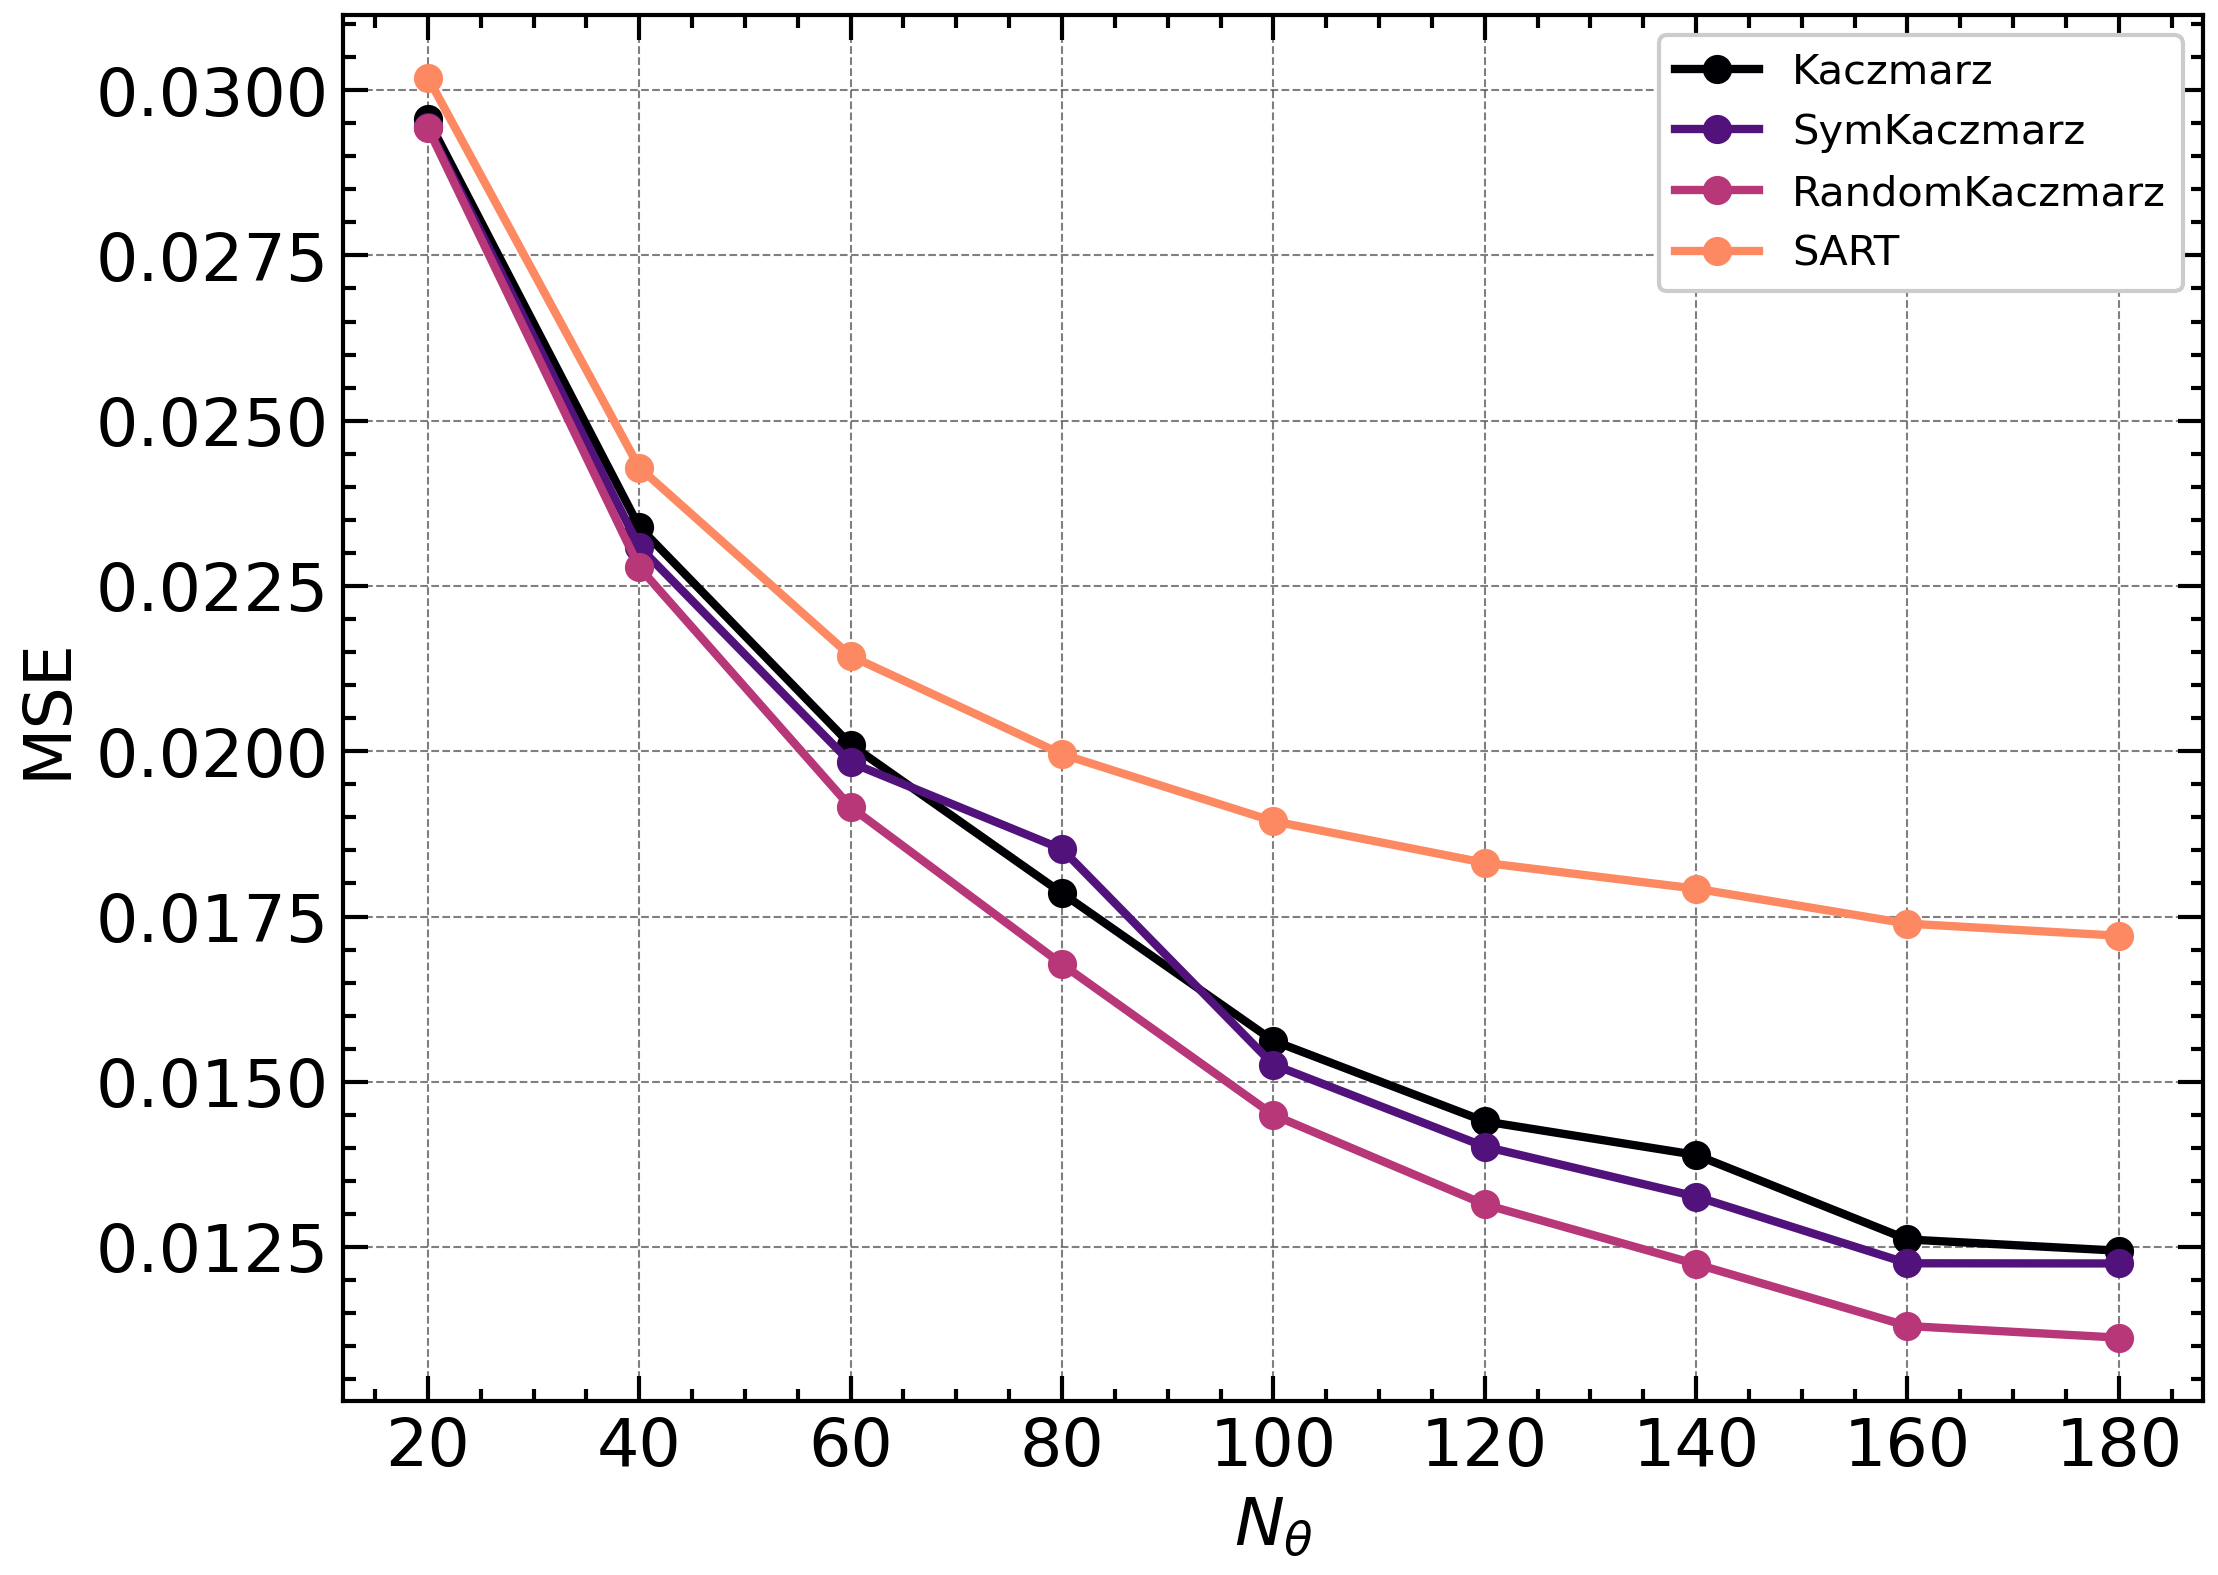
\includegraphics[width=0.45\textwidth]{images/ej_2/angles/mse.png}\label{fig:mse_angles}}
  \hfill
  \subfloat[]{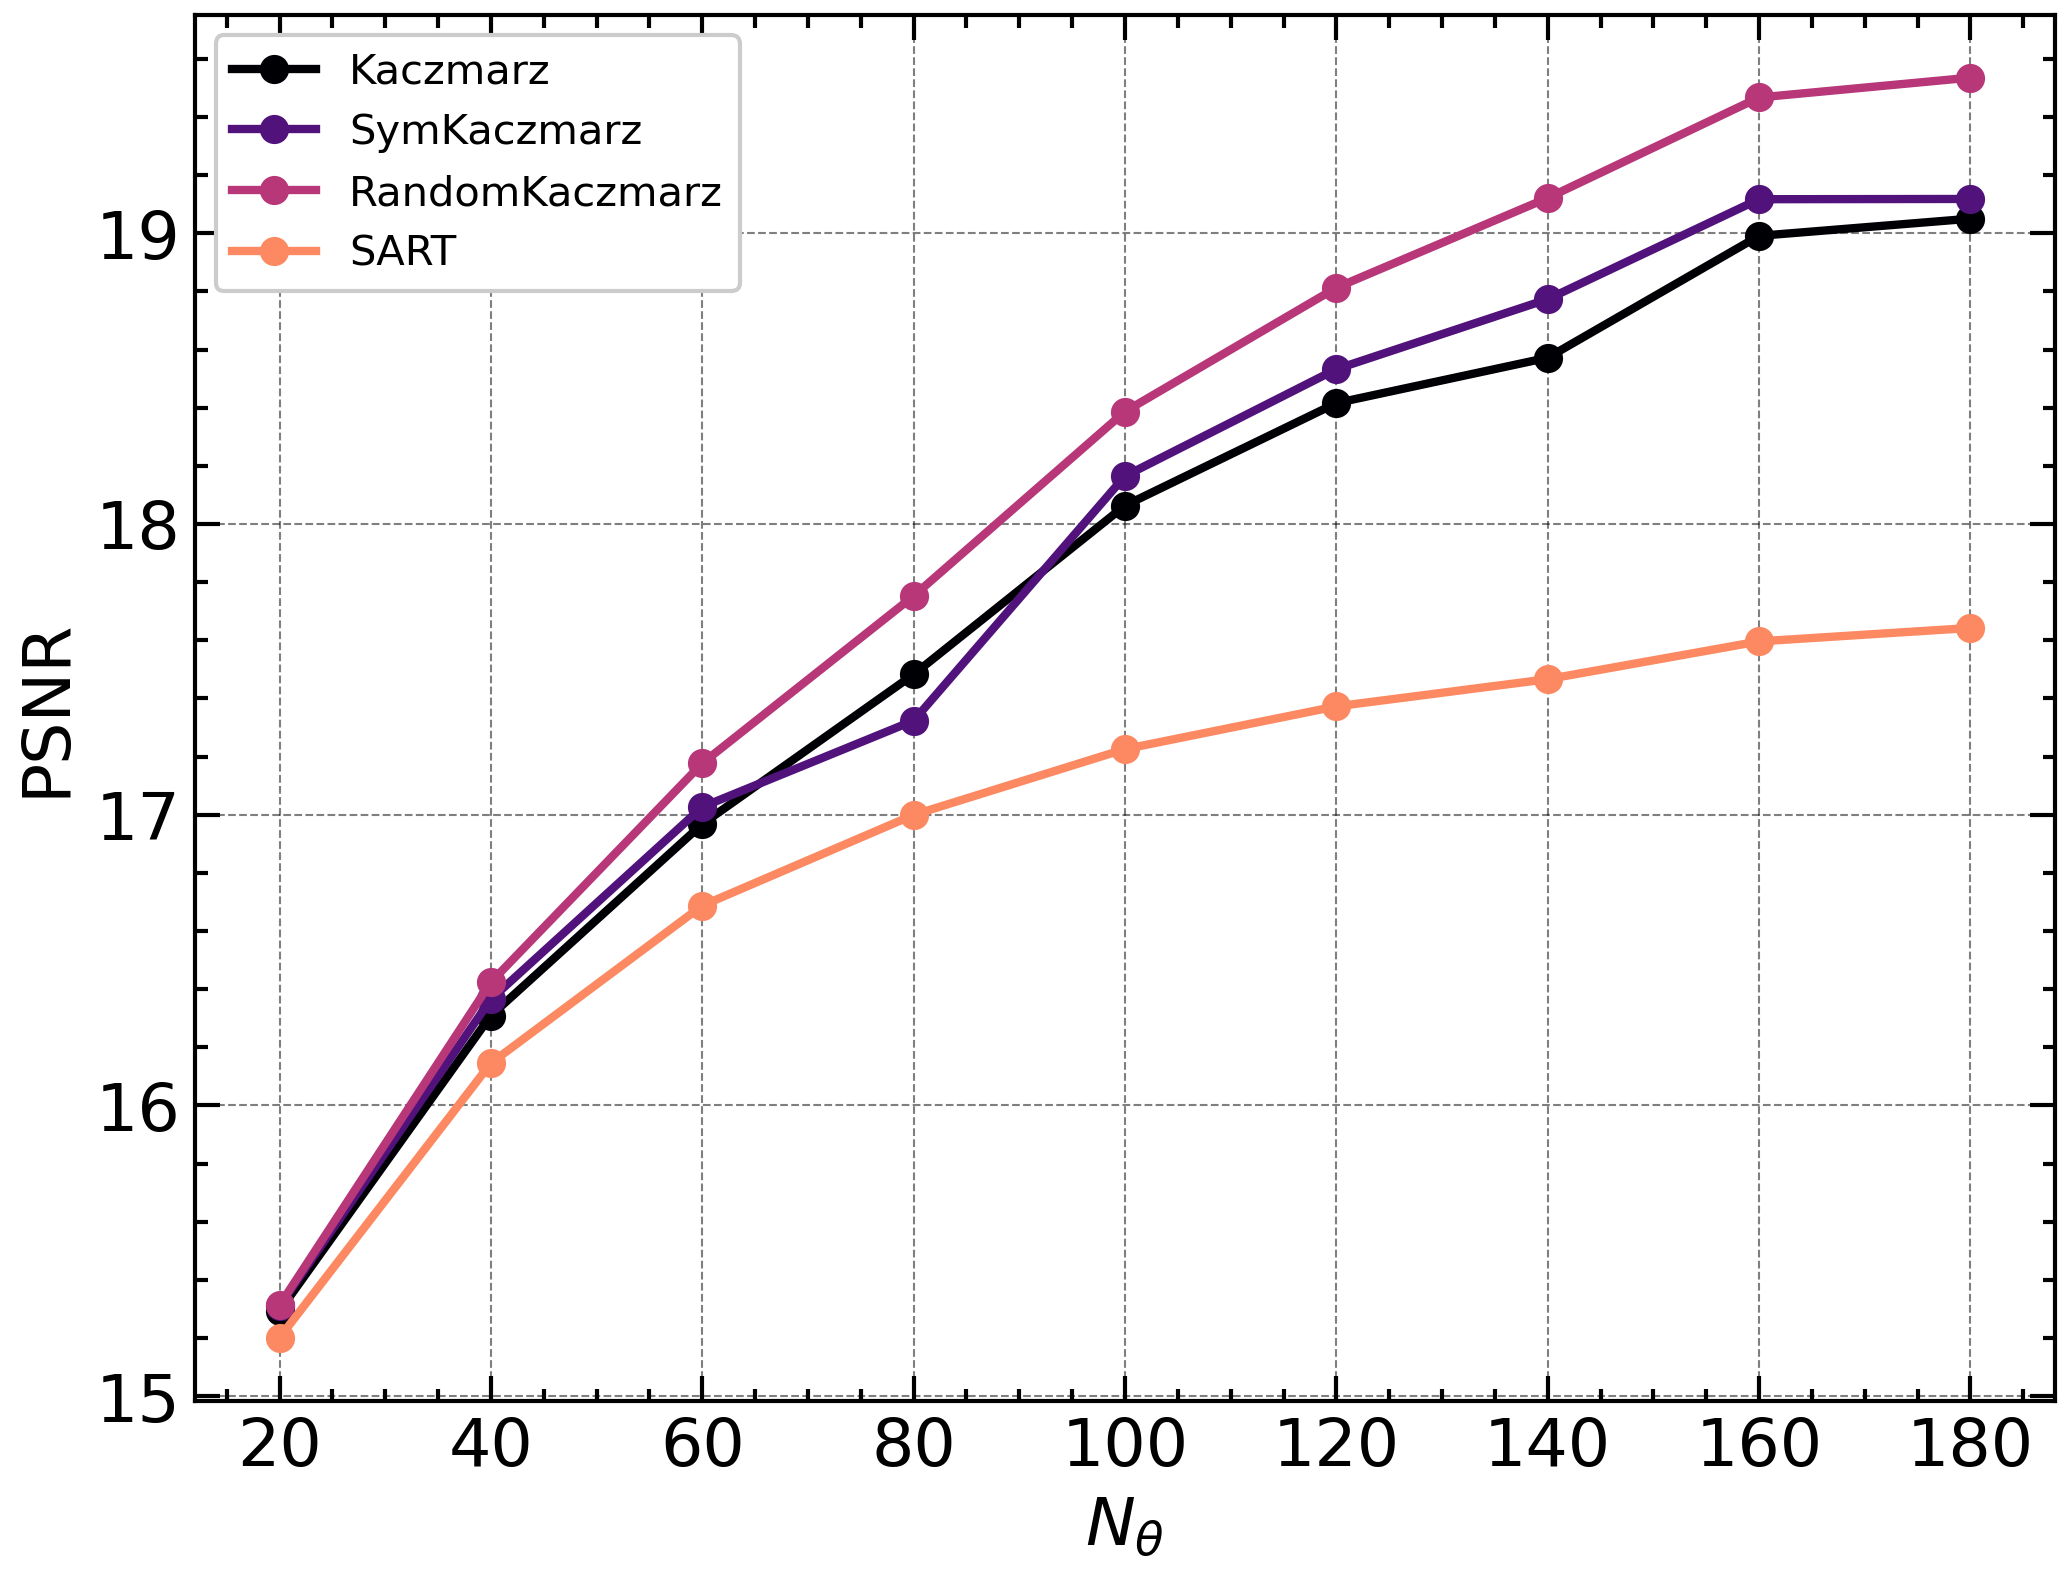
\includegraphics[width=0.42\textwidth]{images/ej_2/angles/psnr.png}\label{fig:psnr_angles}}
  \hfill
  \subfloat[]{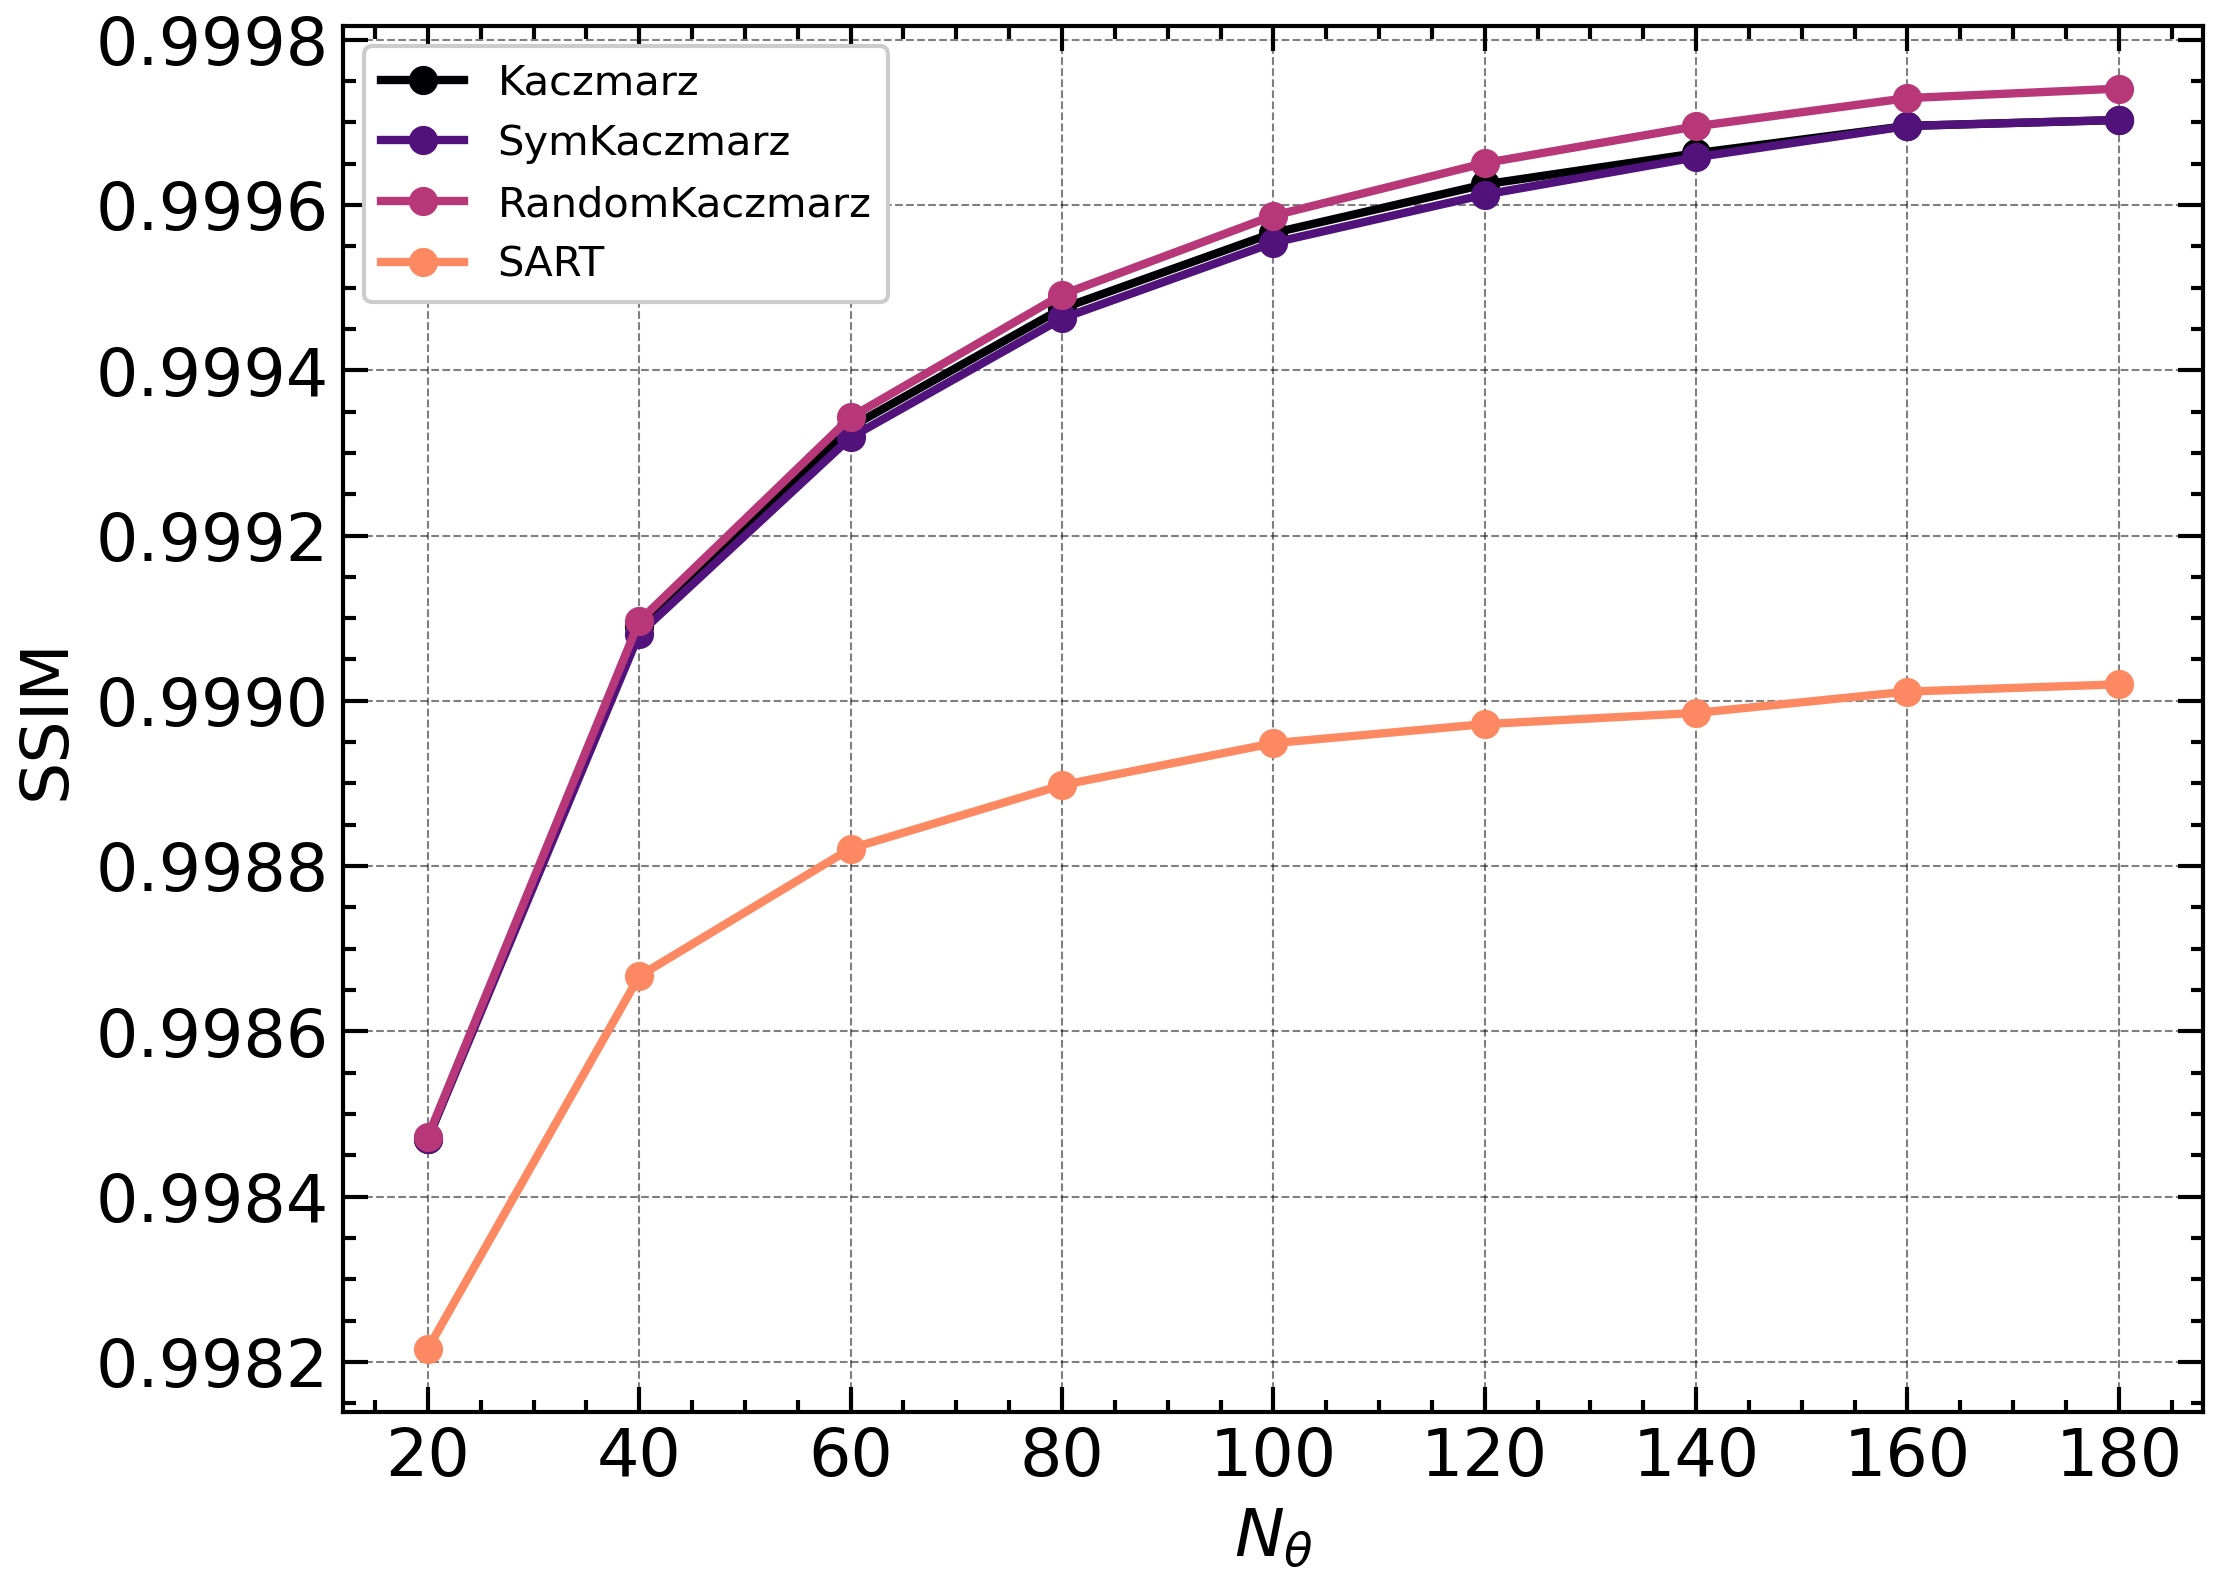
\includegraphics[width=0.45\textwidth]{images/ej_2/angles/ssim.png}\label{fig:ssim_angles}}
  \hfill
  \caption{error de reconstrucción de la imagen original según el número de ángulos ($N_\theta$). (a) Error cuadrático medio (MSE), (b) relación señal a ruido máxima (PSNR), (c) índice de similitud estructural (SSIM).}
  \label{fig:ej_2_angles}
\end{figure}

En la Figura \ref{fig:ej_2_angles}, al aumentar los ángulos, el error \textit{MSE} disminuye (Figura \ref{fig:mse_angles}), mientras que tanto el \textit{PSNR} (Figura \ref{fig:psnr_angles}) como el \textit{SSIM} (Figura \ref{fig:ssim_angles}) aumentan. Esto sugiere una mayor similitud entre la imagen reconstruida y la original con un incremento en el número de ángulos. El algoritmo \textit{SART} muestra una tendencia similar, indicando menor sensibilidad a cambios en el número de ángulos en comparación con otros métodos.

Por último, con el número de ángulos fijo ($N_\theta = 100$) y el número de detectores constante ($N_d = 128$), se varió el nivel de ruido entre 0.01 y 0.1. Los resultados están representados en la Figura \ref{fig:ej_2_noises}.

\begin{figure}[htbp]
  \centering
  \subfloat[]{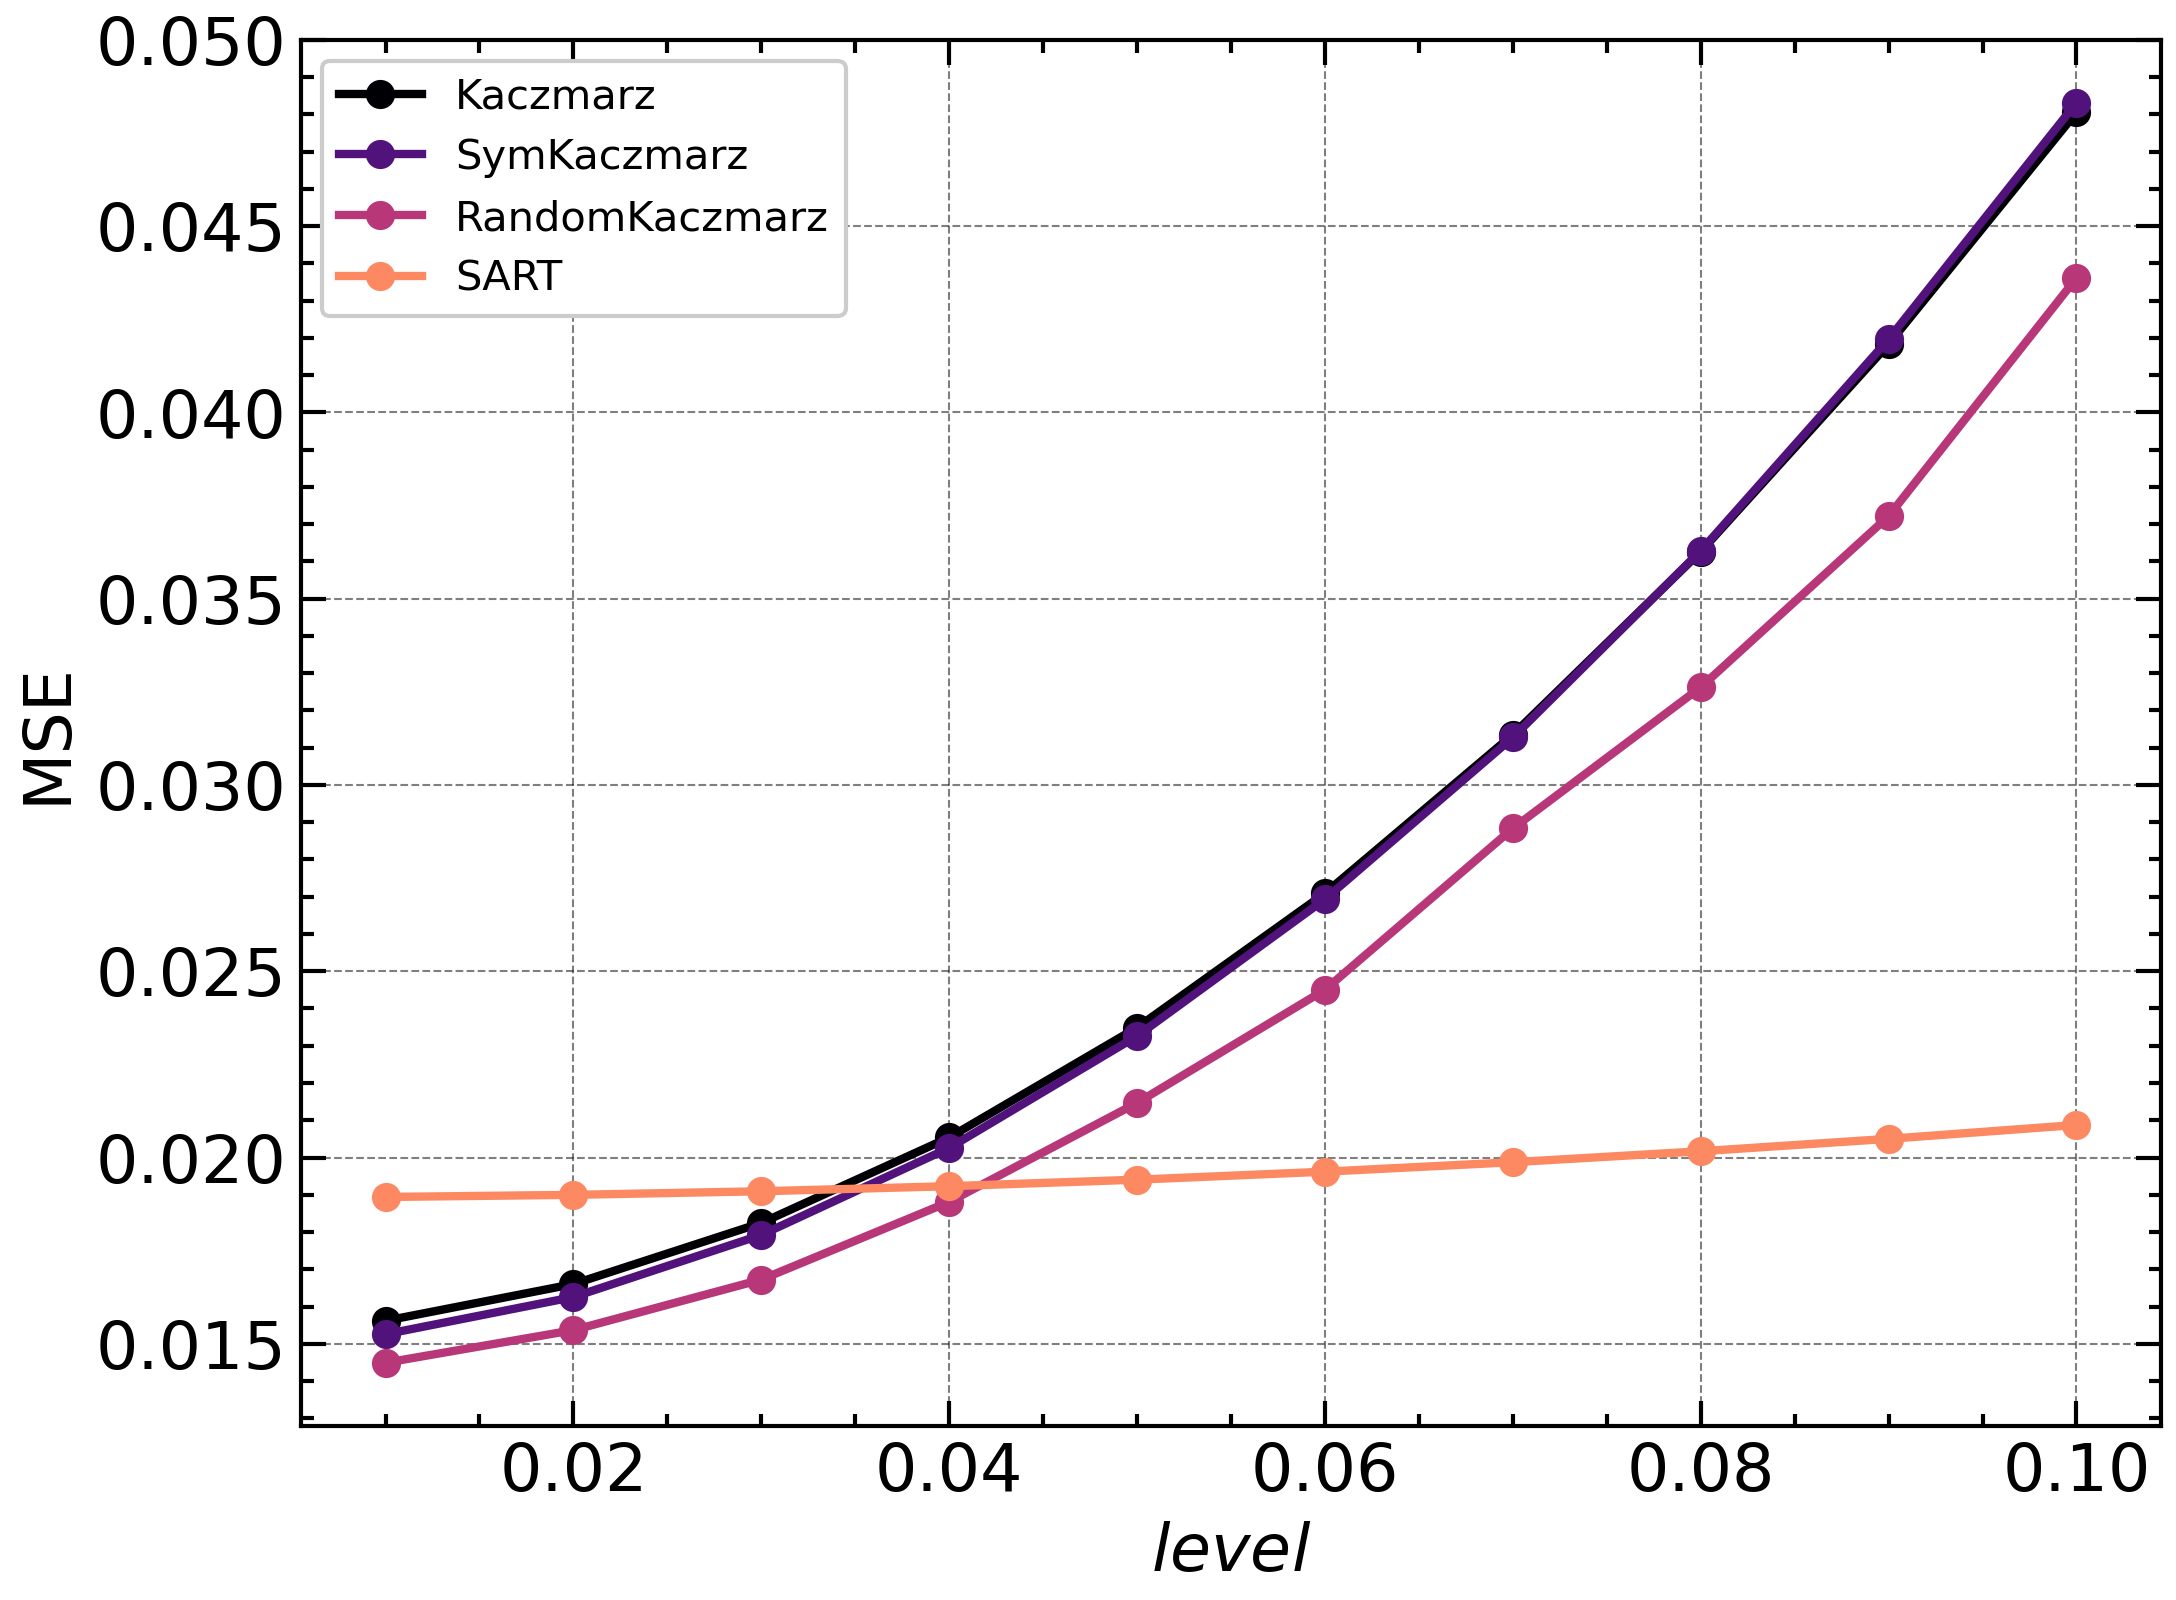
\includegraphics[width=0.45\textwidth]{images/ej_2/noises/mse.png}\label{fig:mse_noises}}
  \hfill
  \subfloat[]{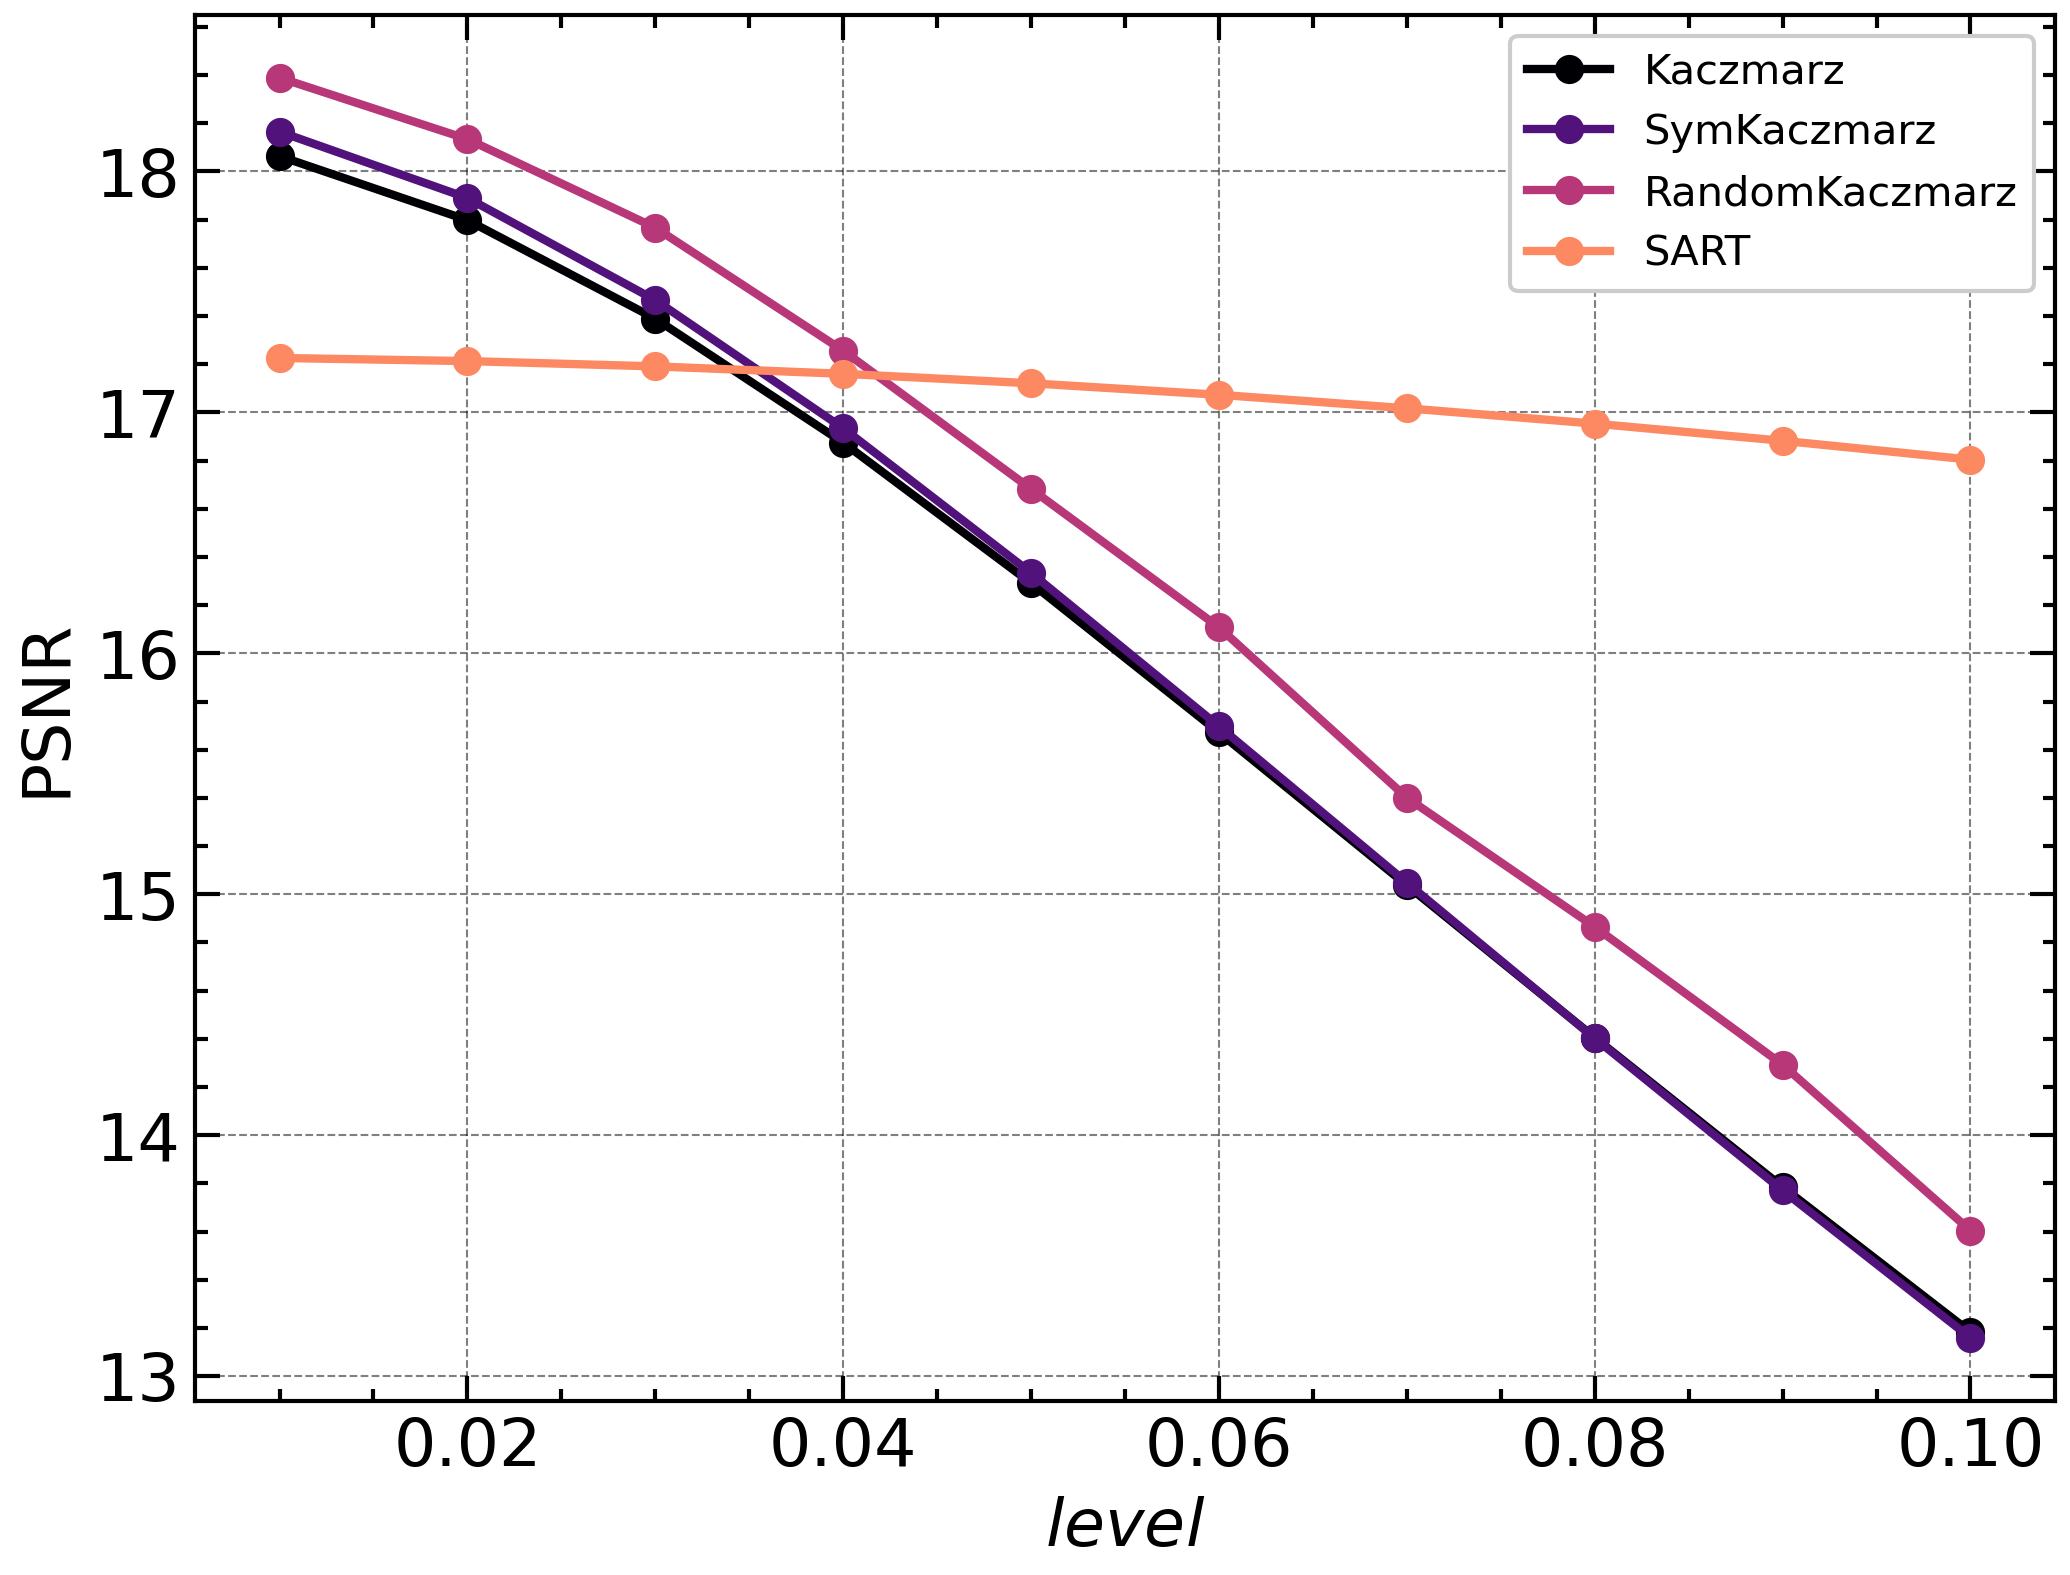
\includegraphics[width=0.42\textwidth]{images/ej_2/noises/psnr.png}\label{fig:psnr_noises}}
  \hfill
  \subfloat[]{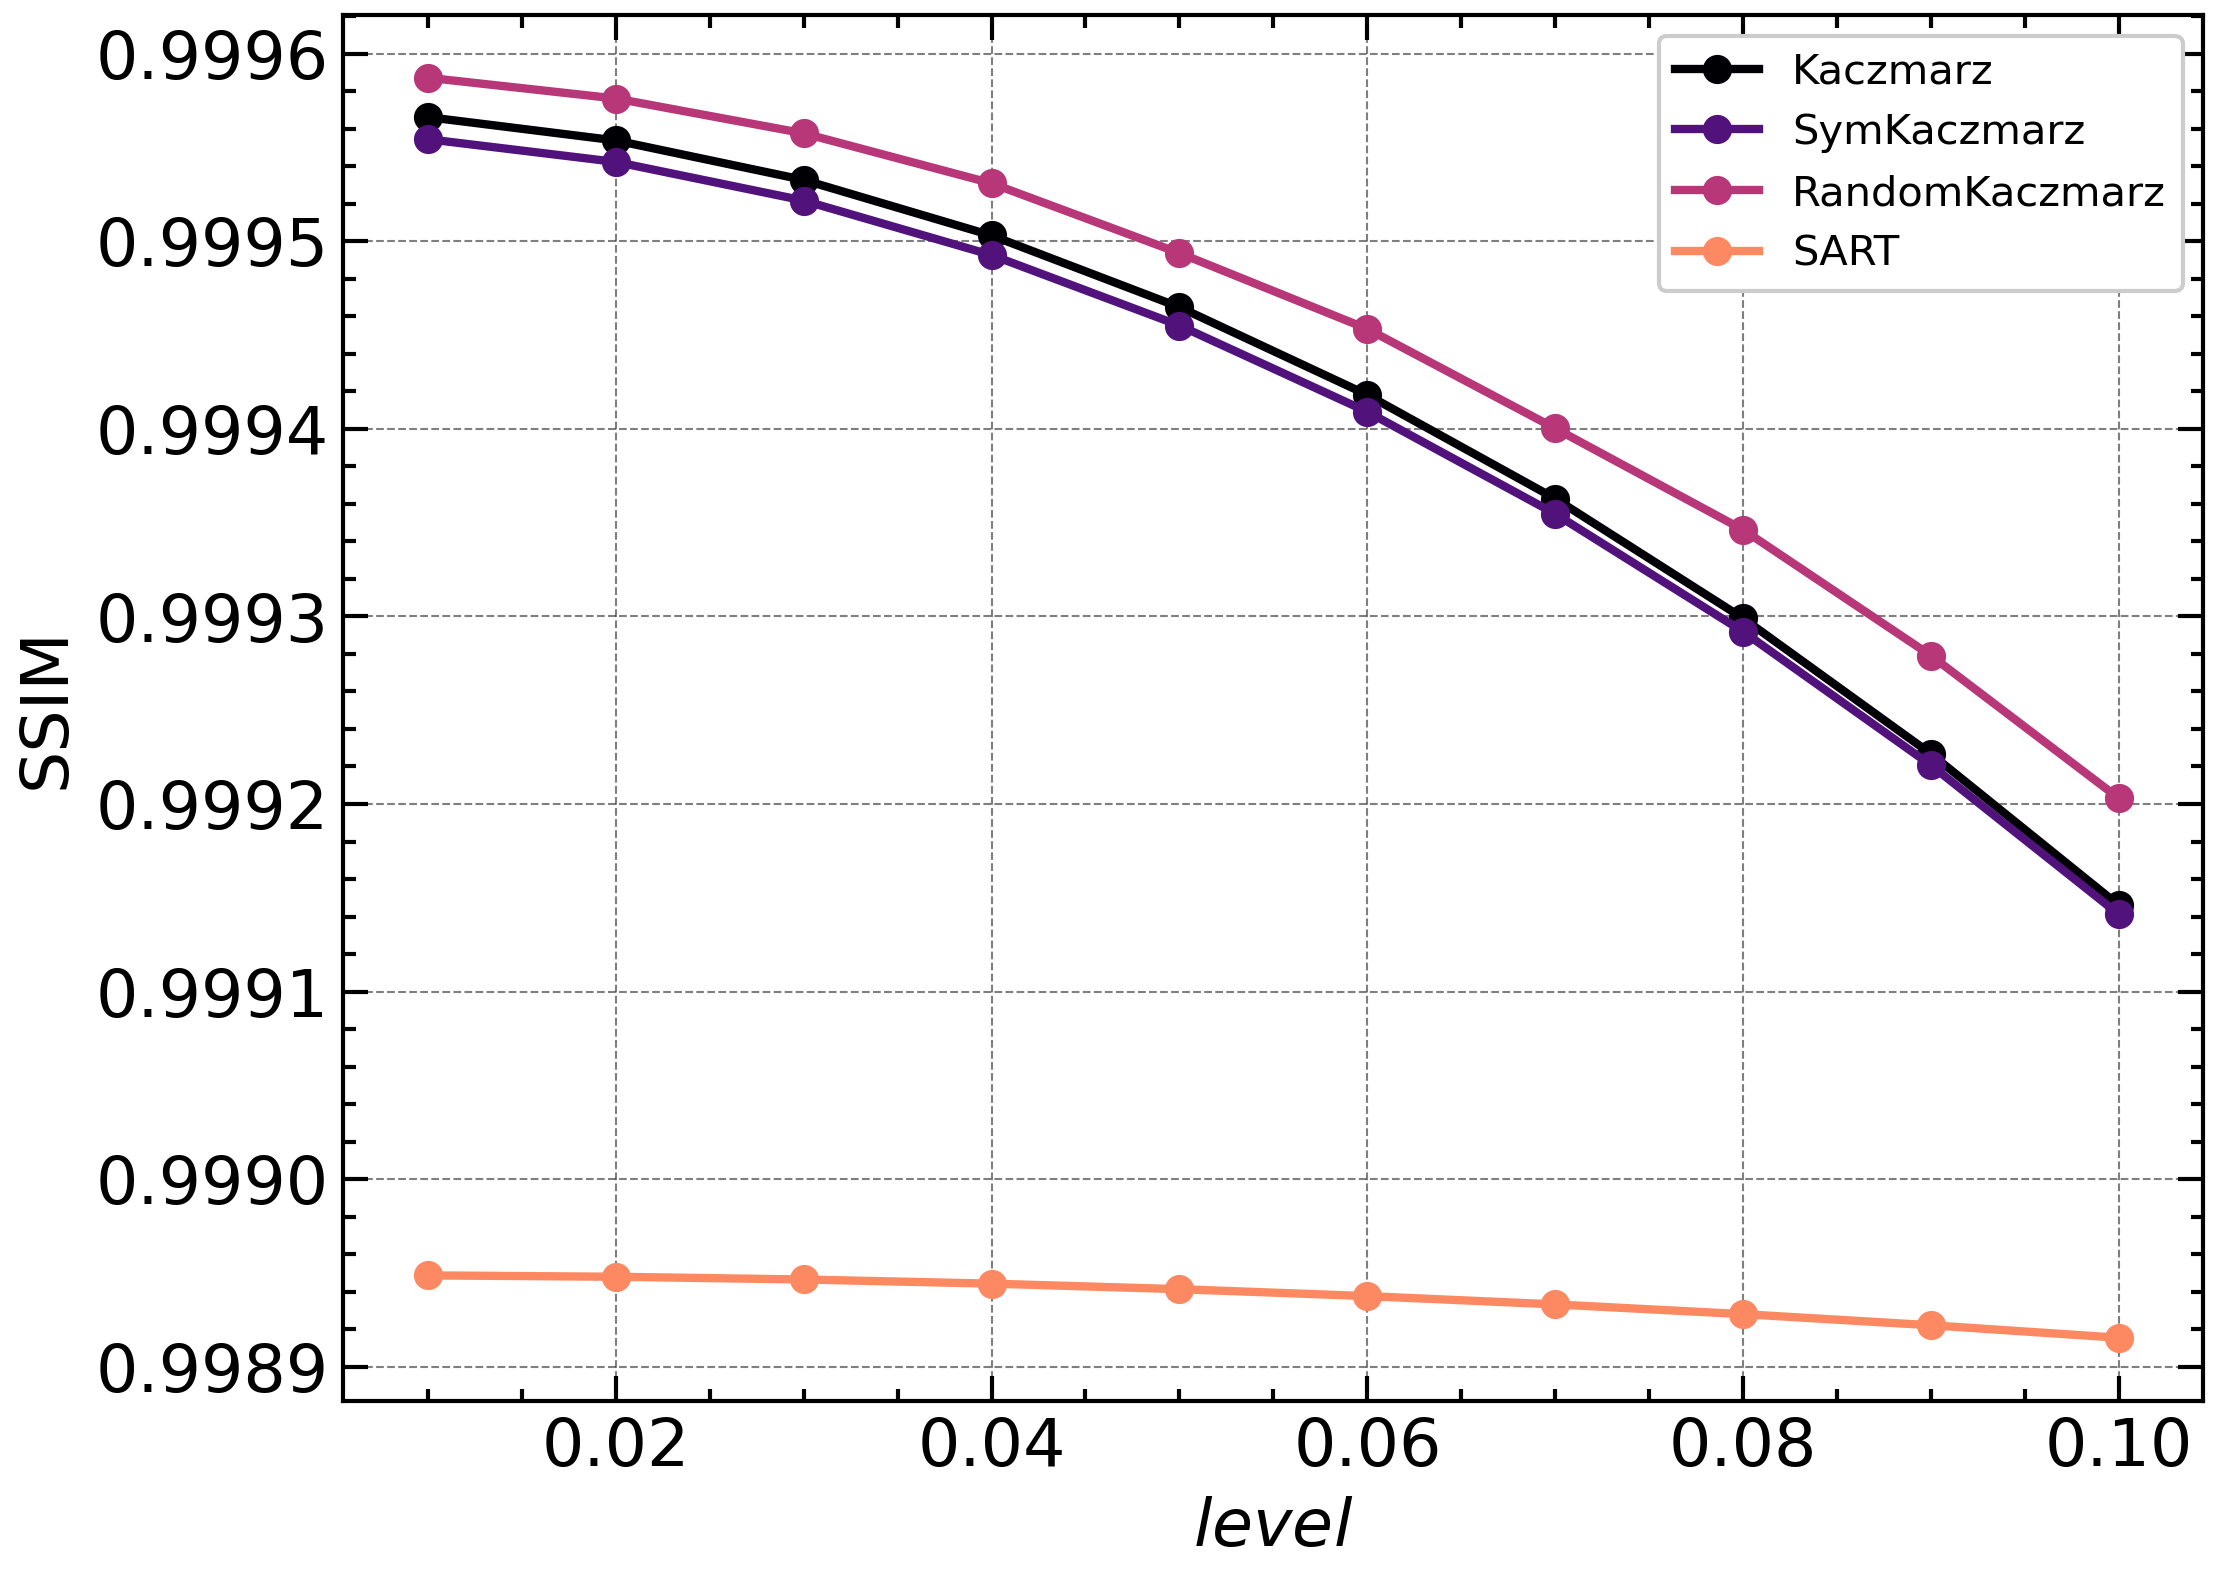
\includegraphics[width=0.45\textwidth]{images/ej_2/noises/ssim.png}\label{fig:ssim_noises}}
  \hfill
  \caption{error de reconstrucción de la imagen original según nivel de ruido ($level$). (a) Error cuadrático medio (MSE), (b) relación señal a ruido máxima (PSNR), (c) índice de similitud estructural (SSIM).}
  \label{fig:ej_2_noises}
\end{figure}

Al aumentar el ruido en la imagen (Figura \ref{fig:ej_2_noises}), se observa un incremento significativo en el error \textit{MSE} (Figura \ref{fig:mse_noises}), acompañado de una disminución tanto en el \textit{PSNR} (Figura \ref{fig:psnr_noises}) como en el \textit{SSIM} (Figura \ref{fig:ssim_noises}). Estos resultados indican de una notable disminución de la calidad de la imagen reconstruida. Sin embargo, se destaca que el algoritmo \textit{SART} presenta una menor sensibilidad al ruido en comparación con otros métodos, lo que sugiere una mayor robustez ante las perturbaciones en las proyecciones.

Además de la calidad de la reconstrucción, se evaluó el tiempo requerido para reconstruir la imagen original según el algoritmo utilizado, en comparación con el tiempo necesario para realizar la transformada de Radón. Este análisis se llevó a cabo manteniendo constantes el número de ángulos ($N_\theta = 100$), el número de detectores ($N_d = 128$), y el tamaño de la imagen de salida ($240\times240$). Cada algoritmo se iteró en 10 ocasiones para obtener una estimación precisa de los tiempos de reconstrucción. Los resultados detallados se presentan en la Tabla \ref{tab:ej_2_times}.

% Al aumentar el ruido en la imagen (Figura \ref{fig:ej_2_noises}), el error \textit{MSE} aumenta (Figura \ref{fig:mse_noises}), mientras que tanto el \textit{PSNR} (Figura \ref{fig:psnr_noises}) como el \textit{SSIM} (Figura \ref{fig:ssim_noises}) disminuyen, indicando una reducción en la calidad de la imagen reconstruida. El algoritmo \textit{SART} muestra una menor sensibilidad al ruido que otros métodos, sugiriendo mayor robustez ante el ruido en las proyecciones.

% Se evaluó también el tiempo de reconstrucción de la imagen original según el algoritmo utilizado, comparado con el tiempo requerido para la transformada de Radón. Manteniendo fijos el número de ángulos ($N_\theta = 100$), el número de detectores ($N_d = 128$), y el tamaño de la imagen de salida ($240\times240$), cada algoritmo se iteró 10 veces. Los resultados están en la Tabla \ref{tab:ej_2_times}.

\begin{table}[htpb]
  \centering
  \begin{tabular}{|c|c|}
    \hline
    \textbf{Método} & \textbf{Tiempo [s]} \\ \hline
    Kaczmarz & $17.30$ \\ \hline
    Kaczmarz simétrico & $42.82$ \\ \hline
    Kaczmarz aleatorio & $16.00$ \\ \hline
    SART & $0.06$ \\ \hline
    Radon & $0.9$ \\ \hline
  \end{tabular}
  \caption{tiempo de reconstrucción de la imagen original según el algoritmo utilizado.}
  \label{tab:ej_2_times}
\end{table}

En la Tabla \ref{tab:ej_2_times}, se destaca la notable diferencia en velocidad entre el algoritmo \textit{SART} y la transformada de Radón, destacando la eficiencia del primero frente a los algoritmos \textit{Kaczmarz}, siendo el \textit{Kaczmarz simétrico} el más lento. Esta diferencia en la velocidad se atribuye a la capacidad del algoritmo \textit{SART} para actualizar simultáneamente todos los píxeles de la imagen, en contraste con los métodos secuenciales como los algoritmos \textit{Kaczmarz}.

Por otro lado, se realizó la reconstrucción del fantoma de \textit{Shepp-Logan} empleando el algoritmo \textit{Expectation Maximization} (\textit{EM}), con el propósito de evaluar su convergencia en función del número de iteraciones. Utilizando un script de \texttt{Matlab}, se generó la imagen reconstruida, manteniendo constantes el número de ángulos ($N_\theta = 100$), el número de detectores ($N_d = 128$) y el tamaño de la imagen de salida. La Figura \ref{fig:ej_2_em} muestra el proceso de reconstrucción luego de haberse realizado $10$ iteraciones.


\begin{figure}[htbp]
  \centering
  \subfloat[]{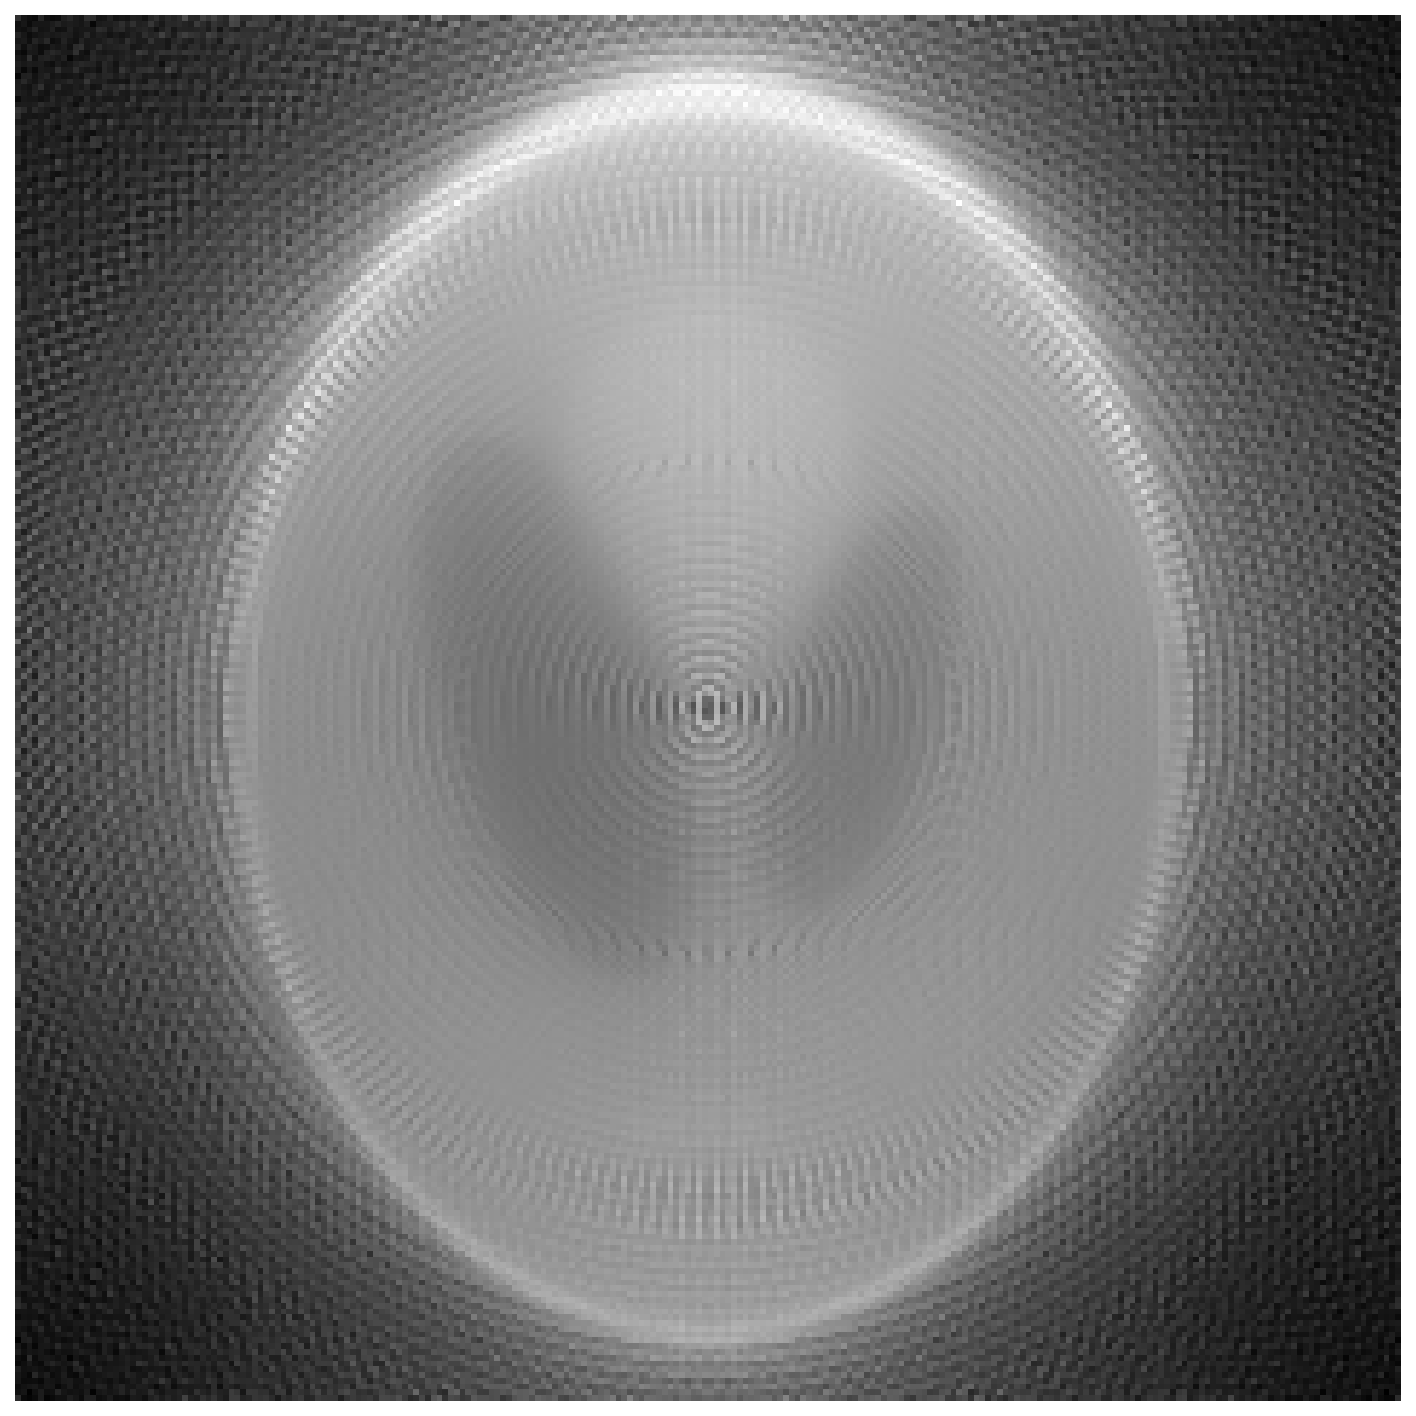
\includegraphics[width=0.24\textwidth]{images/ej_2/exp_max/em_it_0.png}\label{fig:em_it_0}}
  \hfill
  \subfloat[]{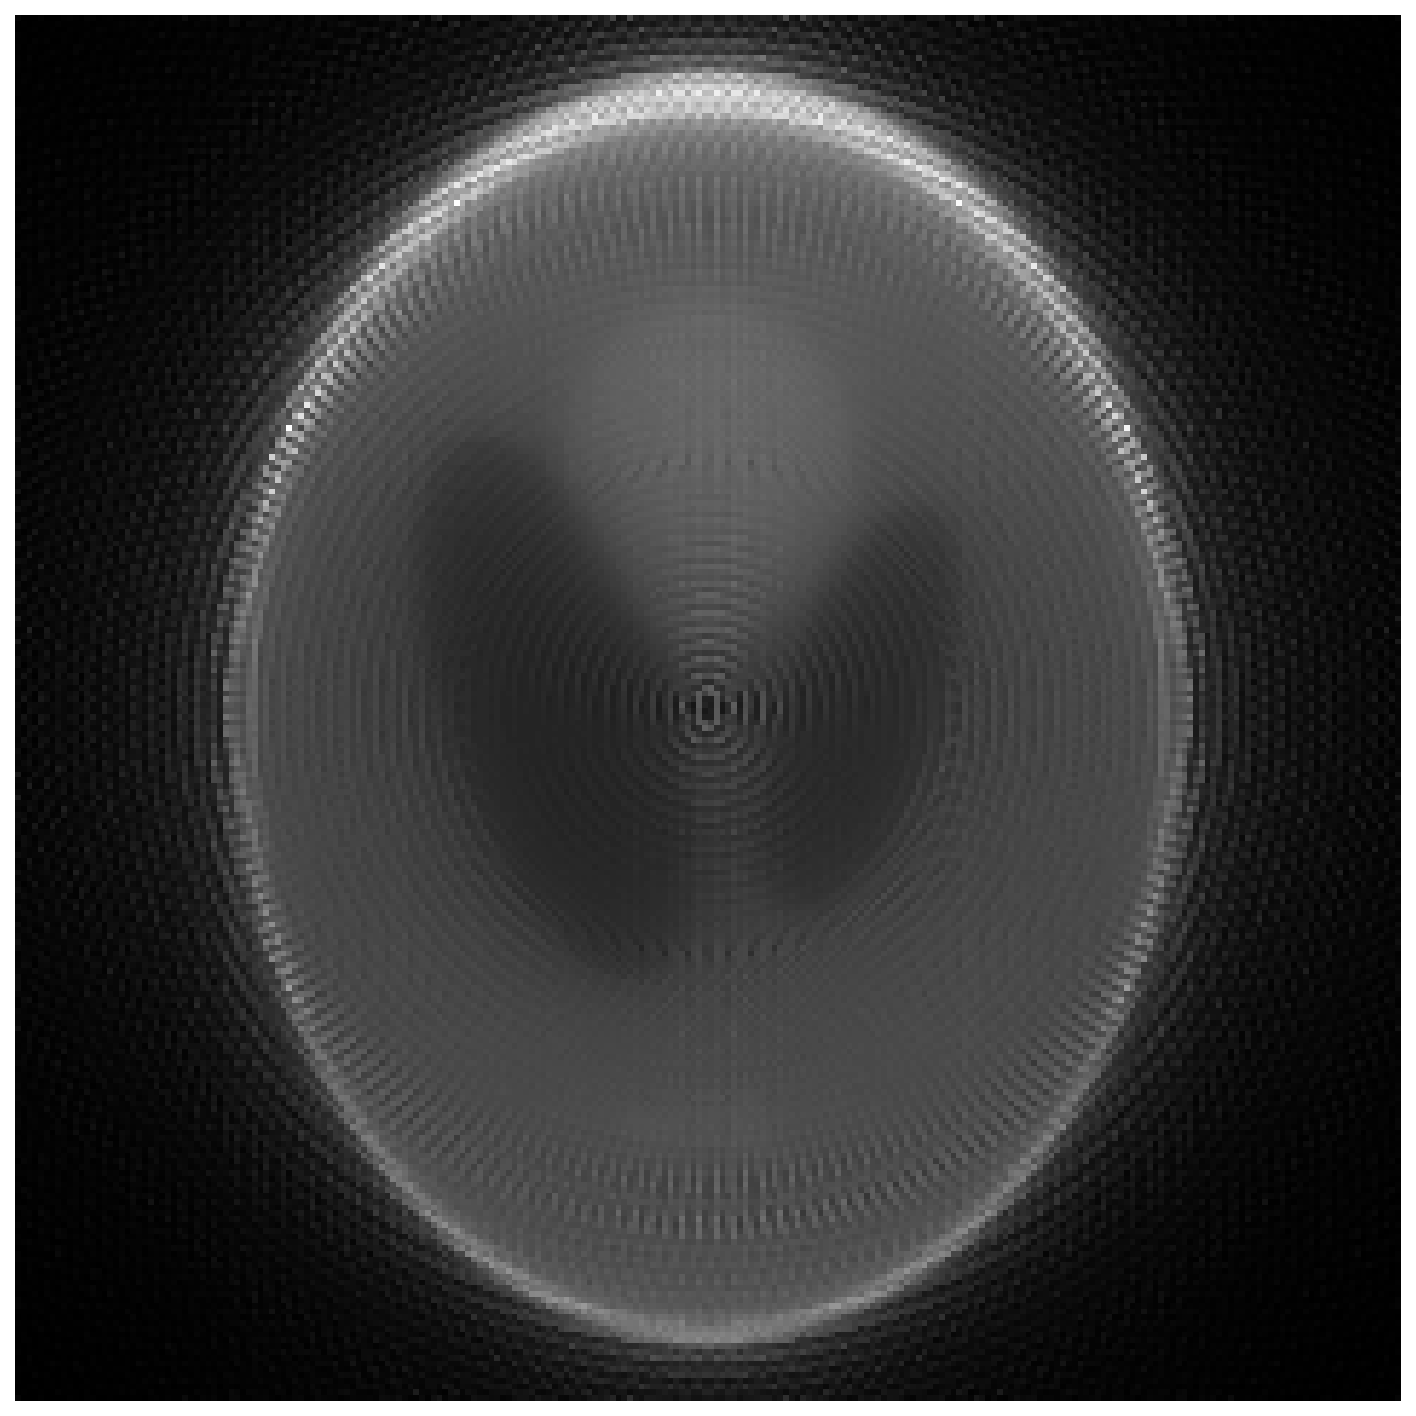
\includegraphics[width=0.24\textwidth]{images/ej_2/exp_max/em_it_3.png}\label{fig:em_it_3}}
  \hfill
  \subfloat[]{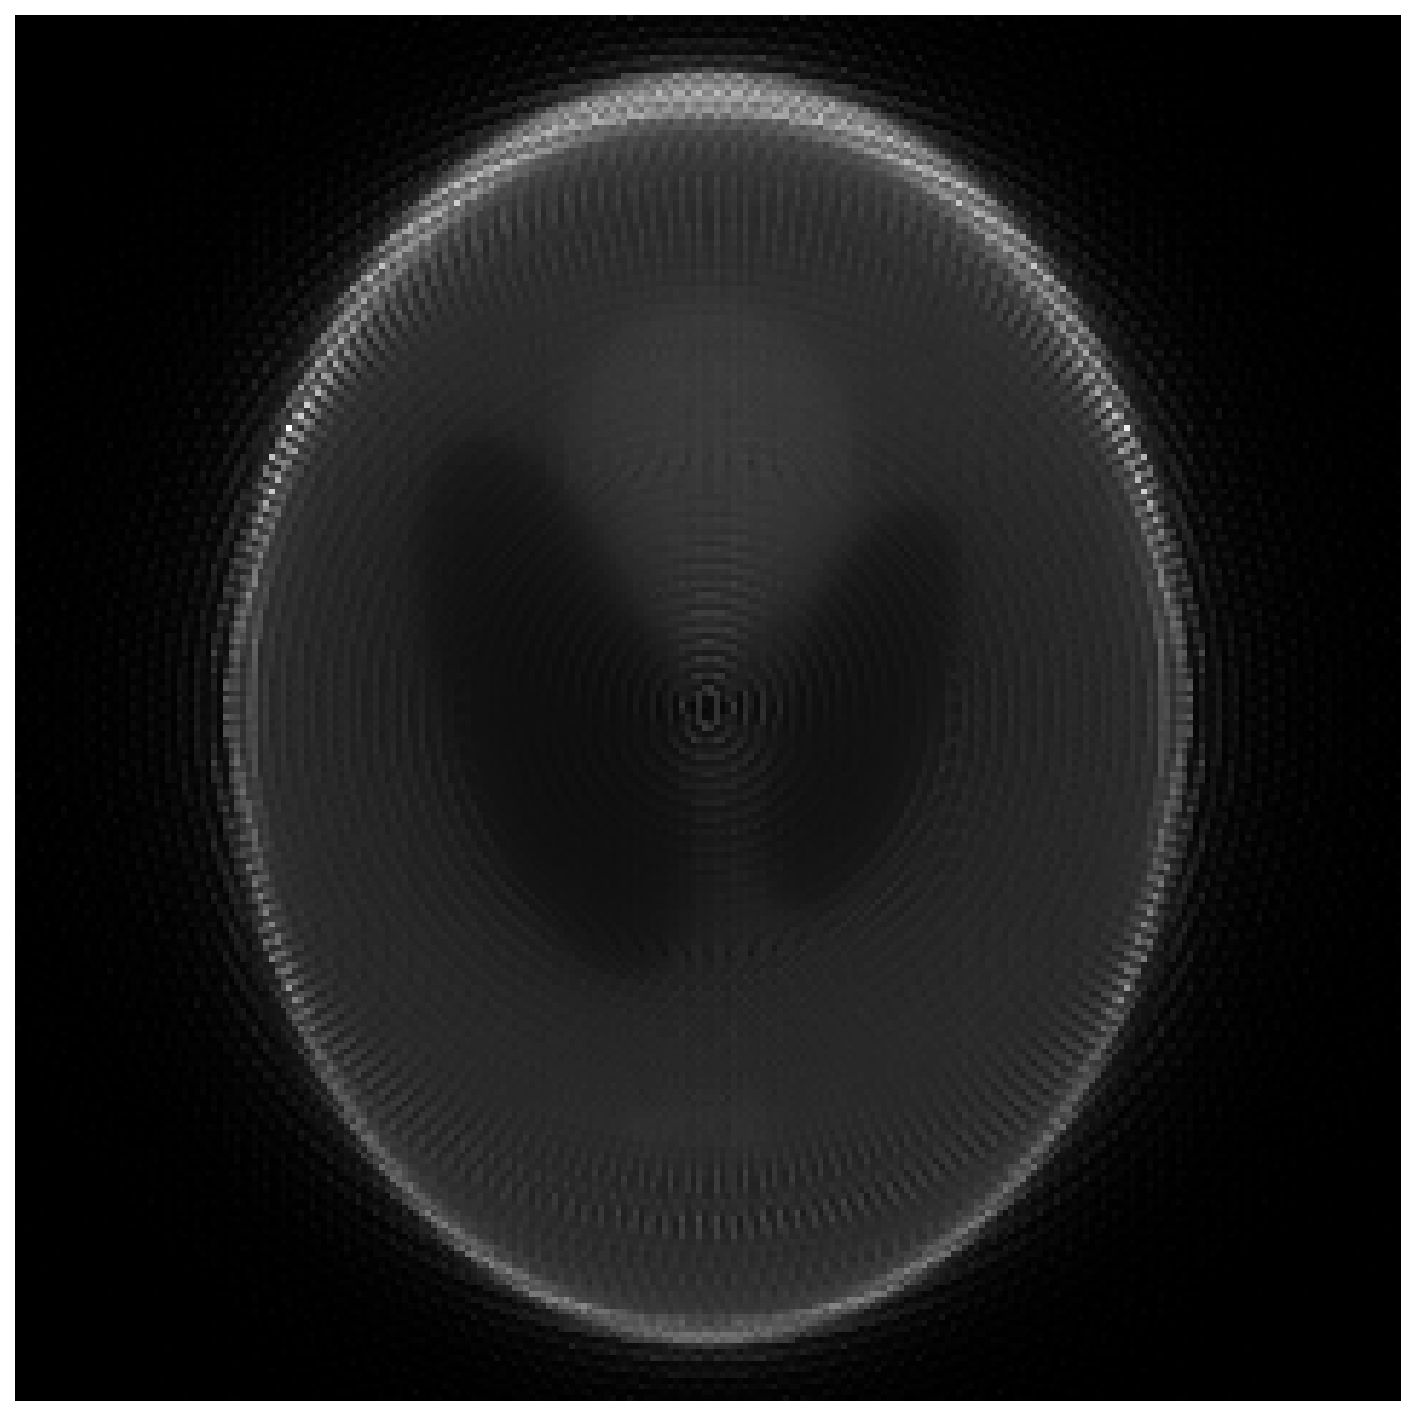
\includegraphics[width=0.24\textwidth]{images/ej_2/exp_max/em_it_6.png}\label{fig:em_it_6}}
  \hfill
  \subfloat[]{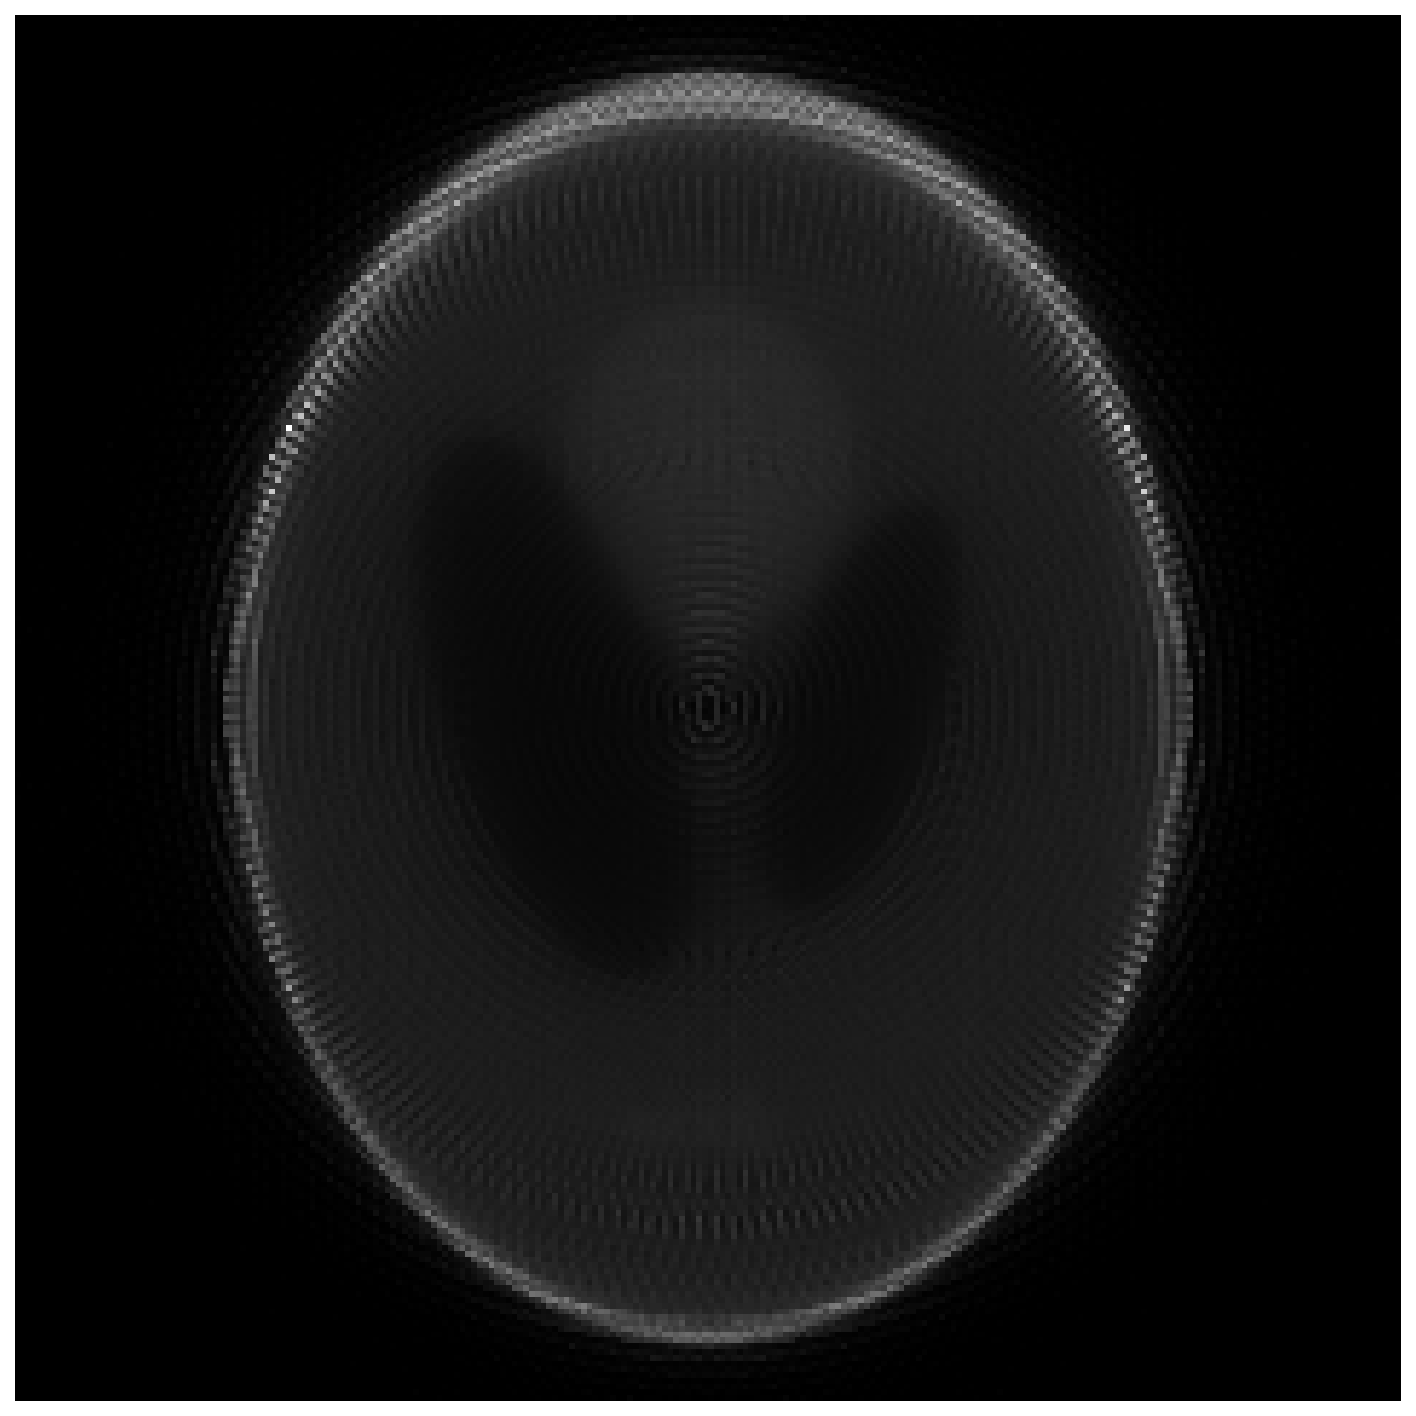
\includegraphics[width=0.24\textwidth]{images/ej_2/exp_max/em_it_9.png}\label{fig:em_it_9}}
  \hfill
  \caption{proceso de reconstrucción del fantoma de Shepp-Logan utilizando el algoritmo Expectation Maximization después de $10$ iteraciones. (a) $1$ iteración, (b) $4$ iteraciones, (c) $7$ iteraciones, (d) $10$ iteraciones.}
  \label{fig:ej_2_em}
\end{figure}

En la Figura \ref{fig:ej_2_em}, se puede apreciar que conforme aumenta el número de iteraciones, la imagen experimenta una pérdida de contraste. De forma evidente, la imagen de 4 iteraciones (Figura \ref{fig:em_it_3}) se destaca por su mayor nitidez y contraste. 

Para analizar el error de reconstrucción del algoritmo \textit{Expectation Maximization}, se calculó el error cuadrático medio (MSE), la relación señal a ruido máxima (PSNR) y el índice de similitud estructural (SSIM) según el número de iteraciones. Los resultados obtenidos se muestran en la Figura \ref{fig:ej_2_em_metrics}.

\begin{figure}[htbp]
  \centering
  \subfloat[]{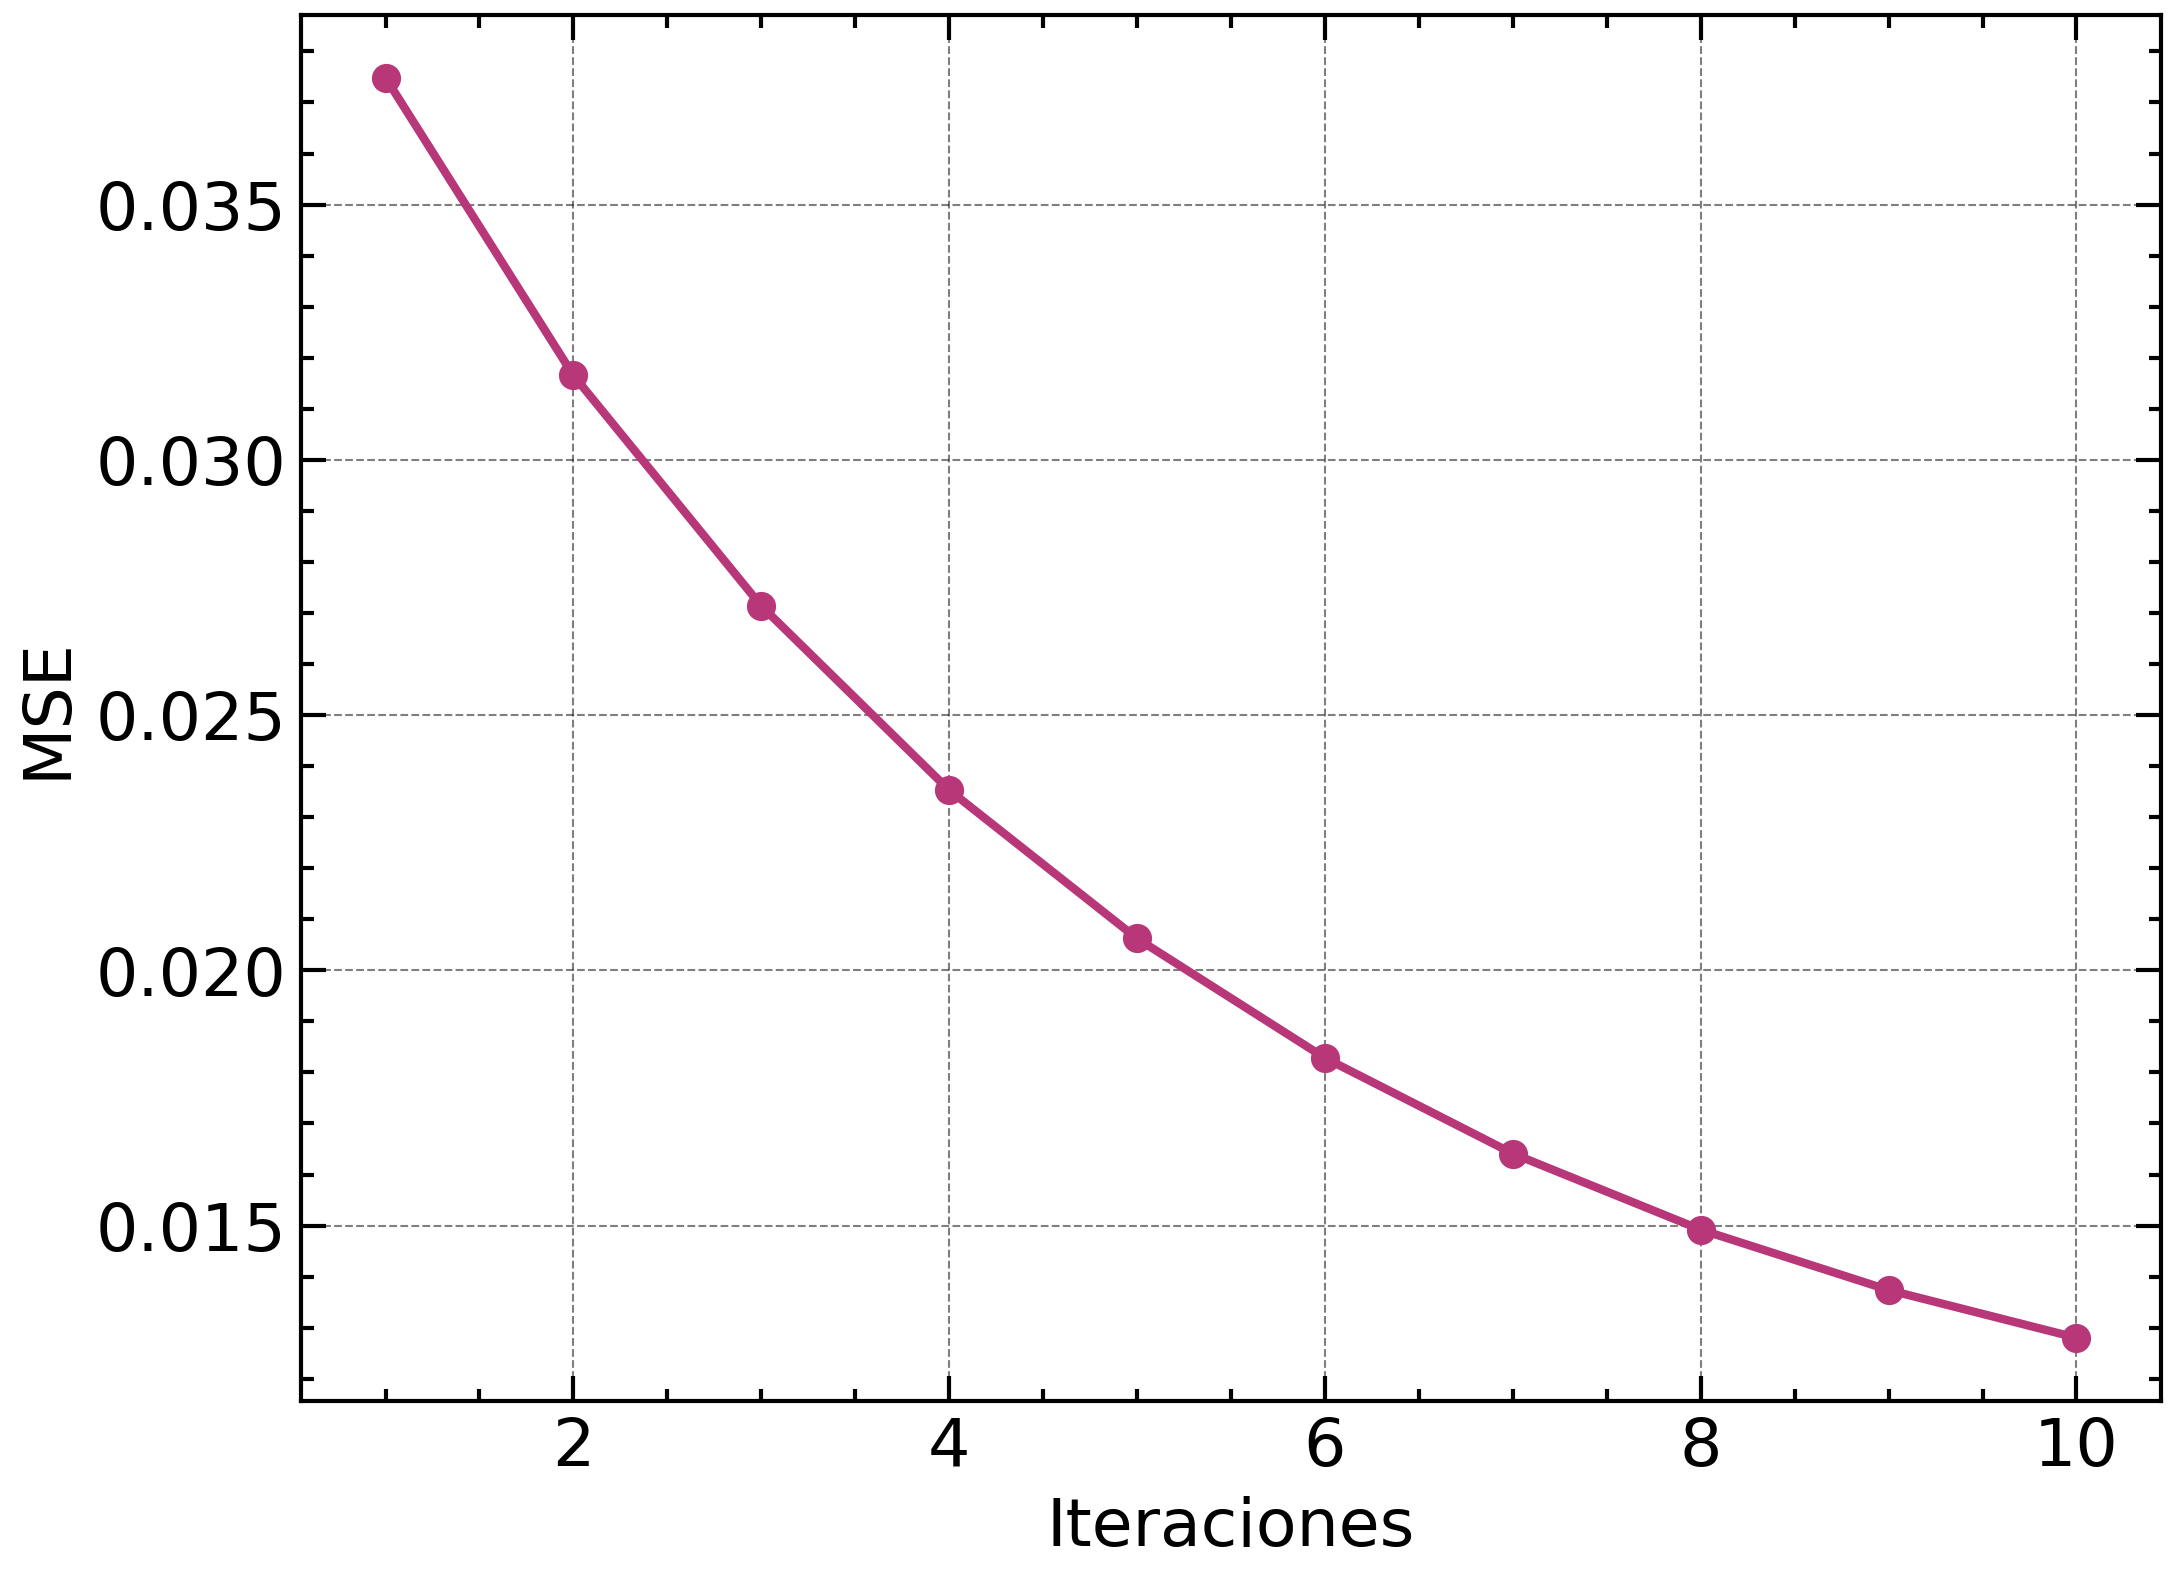
\includegraphics[width=0.45\textwidth]{images/ej_2/exp_max/mse.png}\label{fig:mse_em}}
  \hfill
  \subfloat[]{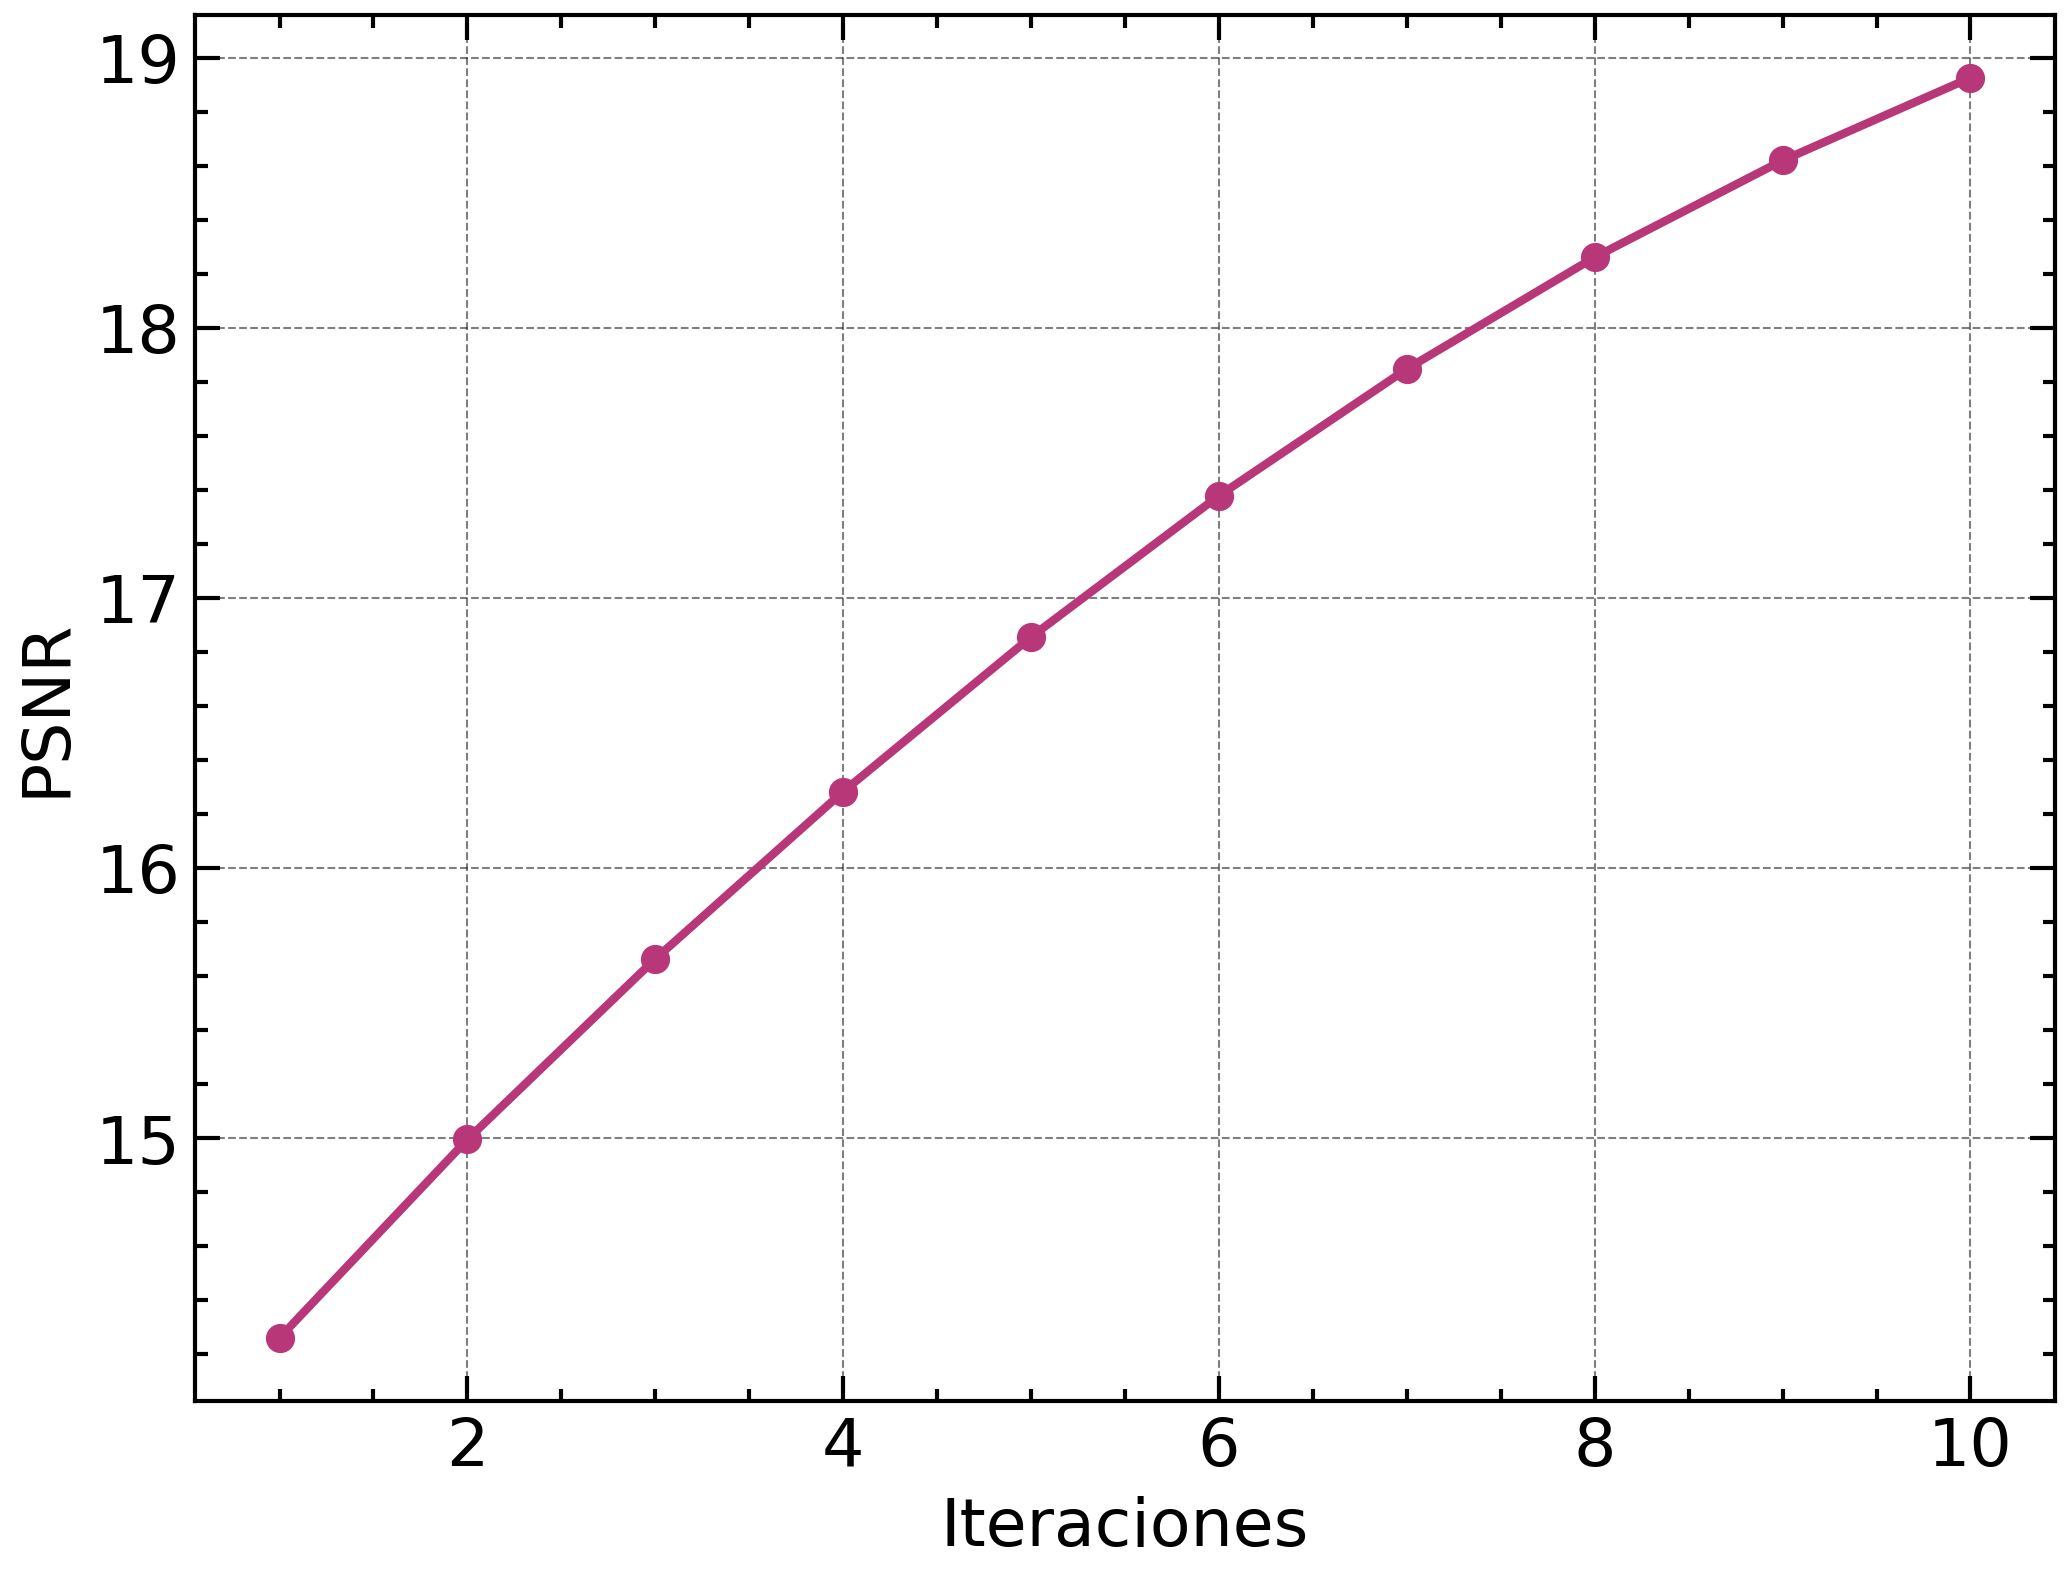
\includegraphics[width=0.40\textwidth]{images/ej_2/exp_max/psnr.png}\label{fig:psnr_em}}
  \hfill
  \subfloat[]{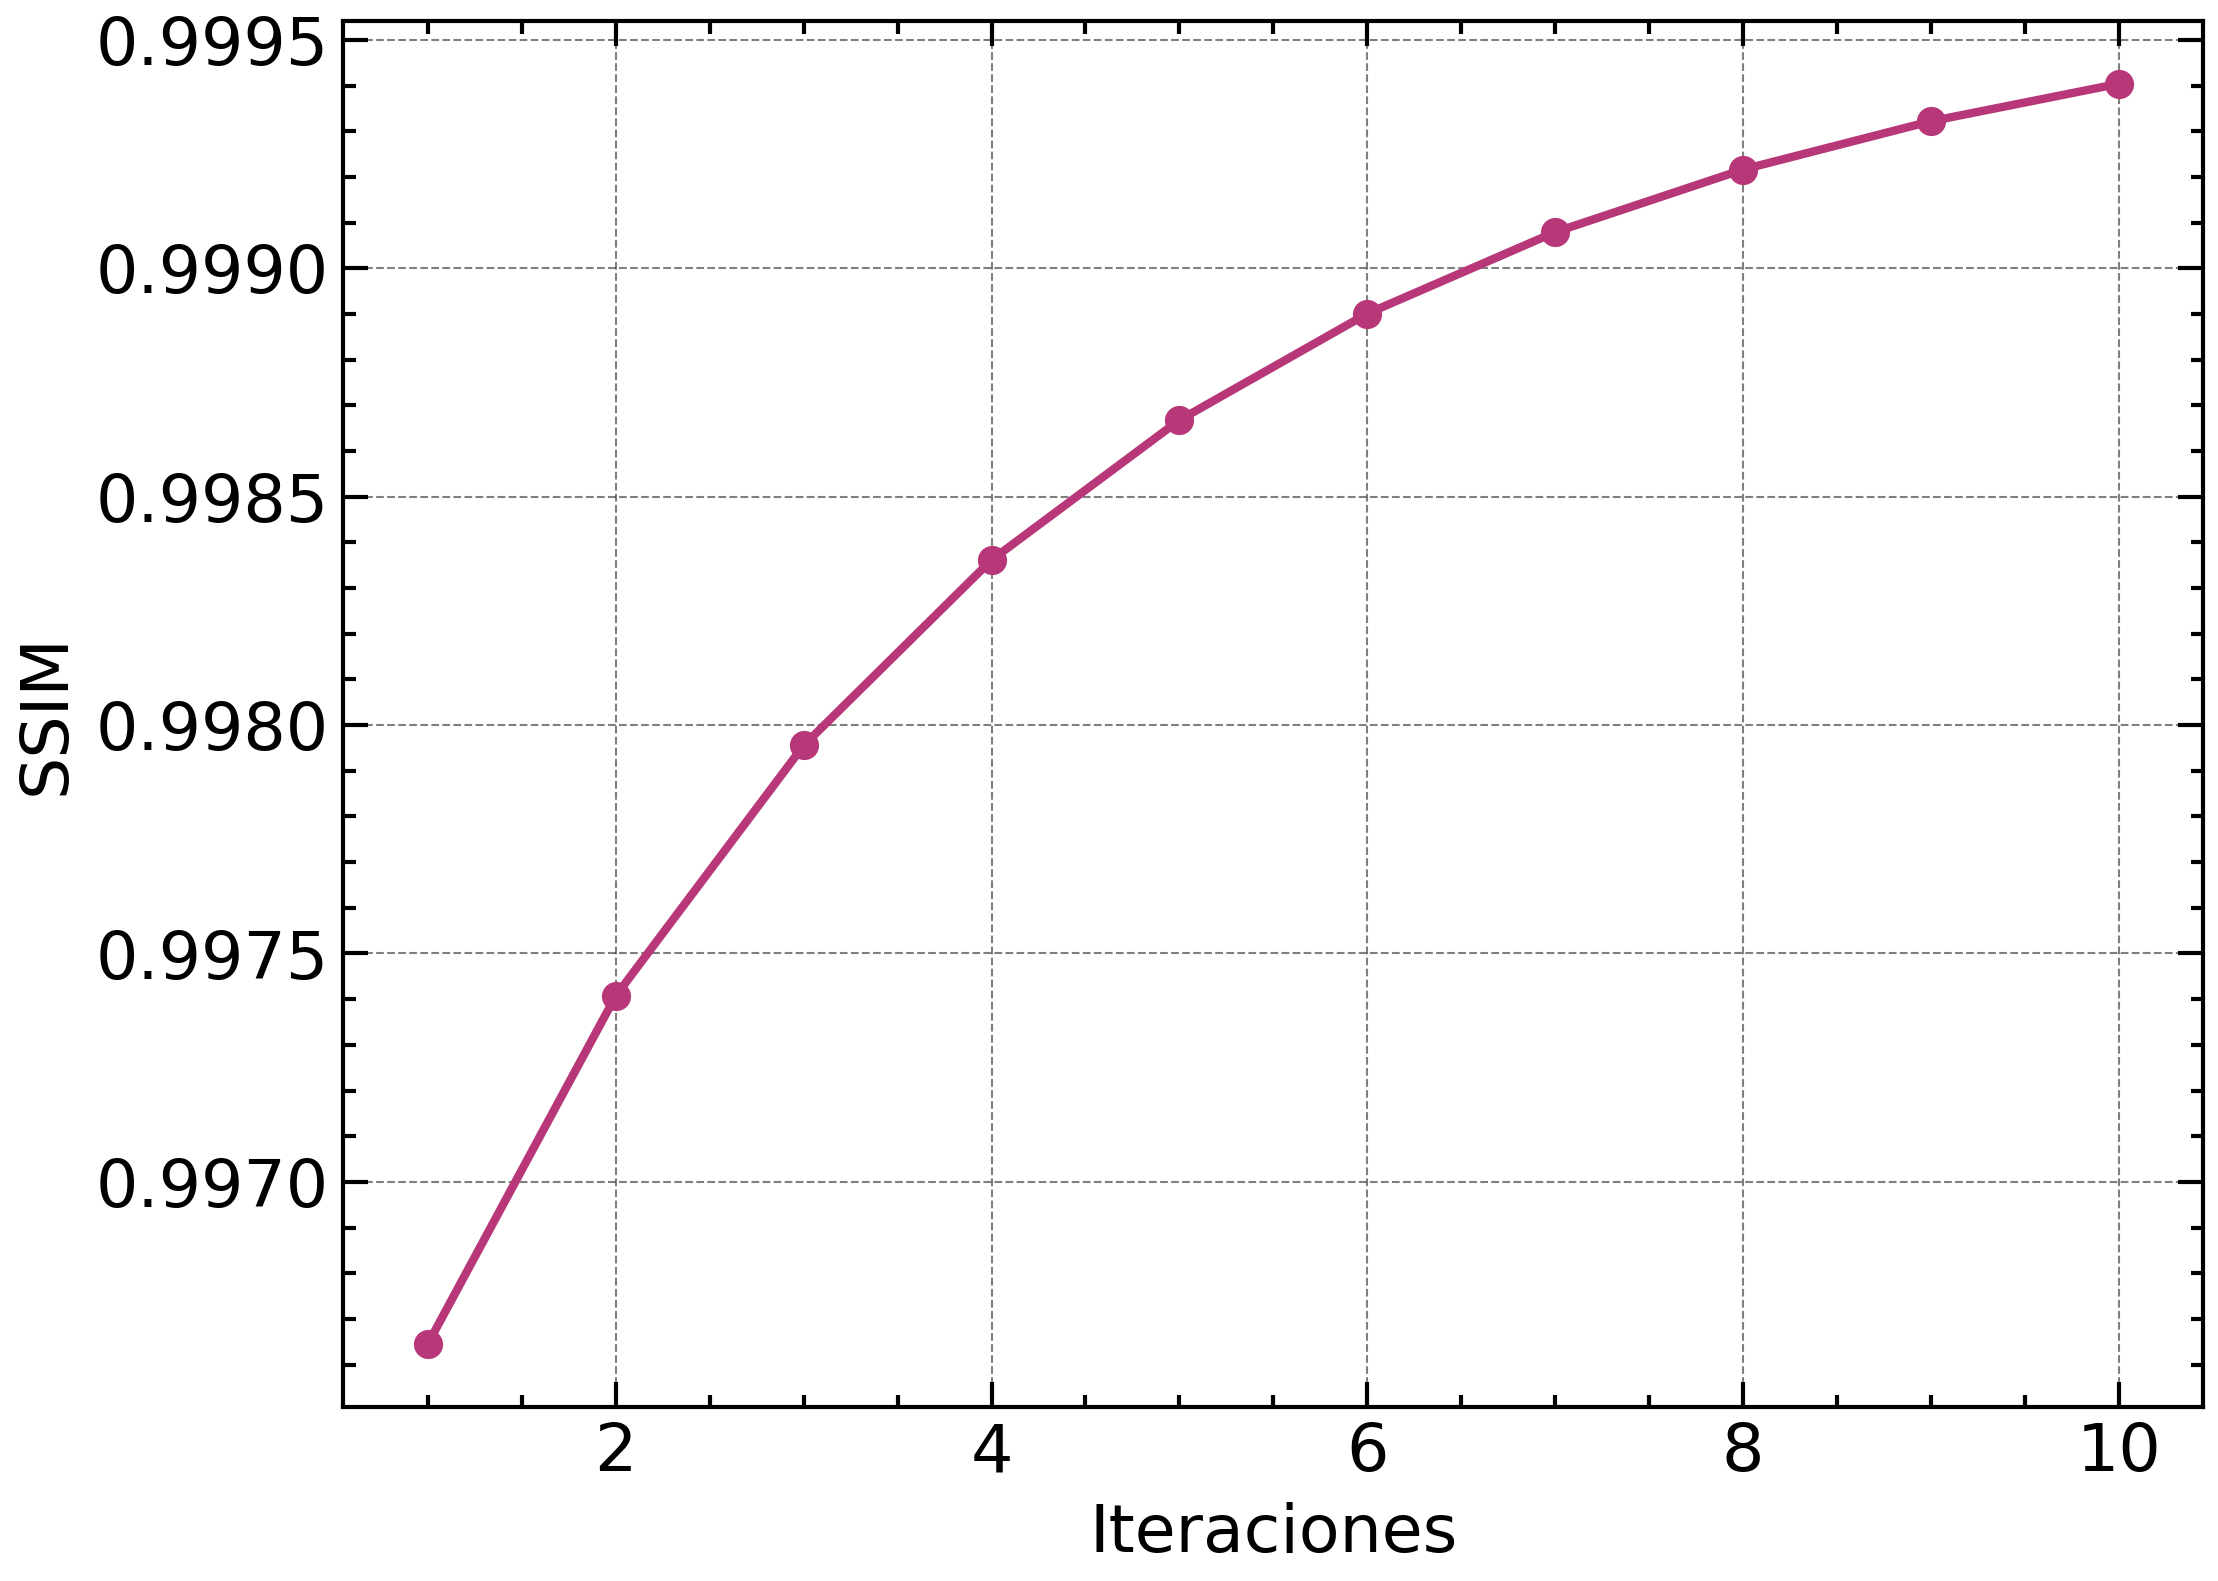
\includegraphics[width=0.45\textwidth]{images/ej_2/exp_max/ssim.png}\label{fig:ssim_em}}
  \hfill
  \caption{error de reconstrucción del fantoma de Shepp-Logan según el número de iteraciones. (a) Error cuadrático medio (MSE), (b) relación señal a ruido máxima (PSNR), (c) índice de similitud estructural (SSIM).}
  \label{fig:ej_2_em_metrics}
\end{figure}

A medida que aumentan las iteraciones, el error \textit{MSE} disminuye (Figura \ref{fig:mse_em}), mientras que tanto el \textit{PSNR} (Figura \ref{fig:psnr_em}) como el \textit{SSIM} (Figura \ref{fig:ssim_em}) aumentan, indicando una mejora en la calidad de la imagen reconstruida. No obstante, es importante tener en cuenta que un incremento de iteraciones puede resultar en una pérdida de contraste y nitidez.

% ------------------ CONCLUSION ---------------------
\section{Conclusiones}
Se llevaron a cabo la implementación y análisis de diversos algoritmos algebraicos para la reconstrucción de imágenes tomográficas, entre ellos \textit{Kaczmarz}, \textit{SART} y \textit{Expectation Maximization}. Se logró evaluar las métricas en cuanto a errores de reconstrucción en cada uno de los casos analizados.

Se evidenció que el algoritmo \textit{ART} mejora la calidad de la imagen a medida que se incrementa el número de iteraciones. Las métricas obtenidas con este método son comparables con aquellas obtenidas mediante la transformada de Radón.

En relación con los análisis realizados, se concluyó que tanto el número de detectores como el de ángulos influyen significativamente en la calidad de la imagen reconstruida, observándose mejoras en las métricas con un aumento en ambos parámetros. Además, se destacó que el algoritmo \textit{SART} demostró ser menos sensible a variaciones en el número de detectores y ángulos en comparación con otros métodos. Asimismo, se observó que el nivel de ruido en las proyecciones impacta la calidad de la reconstrucción, siendo el algoritmo \textit{SART} el más robusto ante esta perturbación.

En cuanto a los tiempos de ejecución, se observó que el algoritmo \textit{SART} fue el más rápido, seguido por la transformada de Radón. Por otro lado, los algoritmos \textit{Kaczmarz} mostraron ser los más lentos, diferenciándose en uno o dos órdenes de magnitud, siendo el \textit{Kaczmarz simétrico} el más lento.

Finalmente, se concluyó que el algoritmo de \textit{Expectation Maximization} es capaz de reconstruir imágenes tomográficas, mejorando sus métricas a medida que se incrementa el número de iteraciones. Sin embargo, se observó visualmente que a partir de cierto número de iteraciones, la imagen puede perder contraste y nitidez.

\end{document}
